\documentclass{report}

%%%%%%%%%%%%%%%%%%%%%%%%%%%%%%%%%
% PACKAGE IMPORTS
%%%%%%%%%%%%%%%%%%%%%%%%%%%%%%%%%
\usepackage[tmargin=2cm,rmargin=1in,lmargin=1in,margin=0.85in,bmargin=2cm,footskip=.2in]{geometry}
\usepackage[none]{hyphenat}
\usepackage{amsmath,amsfonts,amsthm,amssymb,mathtools}
\allowdisplaybreaks
\usepackage{undertilde}
\usepackage{xfrac}
\usepackage[makeroom]{cancel}
\usepackage{mathtools}
\usepackage{bookmark}
\usepackage{enumitem}
\usepackage{kbordermatrix}
\renewcommand{\kbldelim}{(} % Change left delimiter to (
\renewcommand{\kbrdelim}{)} % Change right delimiter to )
\usepackage{hyperref,theoremref}
\hypersetup{
	pdftitle={Assignment},
	colorlinks=true, linkcolor=doc!90,
	bookmarksnumbered=true,
	bookmarksopen=true
}
\usepackage[most,many,breakable]{tcolorbox}
\usepackage{xcolor}
\usepackage{varwidth}
\usepackage{varwidth}
\usepackage{etoolbox}
%\usepackage{authblk}
\usepackage{nameref}
\usepackage{multicol,array}
\usepackage{tikz-cd}
\usepackage[ruled,vlined,linesnumbered]{algorithm2e}
\usepackage{comment} % enables the use of multi-line comments (\ifx \fi) 
\usepackage{import}
\usepackage{xifthen}
\usepackage{pdfpages}
\usepackage{svg}
\usepackage{transparent}
\usepackage{pgfplots}
\pgfplotsset{compat=1.18}
\usetikzlibrary{calc}
\usetikzlibrary{graphs}
\usetikzlibrary{graphs.standard}
% \usetikzlibrary{graphdrawing}

\newcommand\mycommfont[1]{\footnotesize\ttfamily\textcolor{blue}{#1}}
\SetCommentSty{mycommfont}
\newcommand{\incfig}[1]{%
    \def\svgwidth{\columnwidth}
    \import{./figures/}{#1.pdf_tex}
}


\usepackage{tikzsymbols}
% \renewcommand\qedsymbol{$\Laughey$}

\definecolor{commentgreen}{RGB}{2,112,10}
%%
%% Julia definition (c) 2014 Jubobs
%%
\lstdefinelanguage{Julia}%
  {morekeywords={abstract,break,case,catch,const,continue,do,else,elseif,%
      end,export,false,for,function,immutable,import,importall,if,in,%
      macro,module,otherwise,quote,return,switch,true,try,type,typealias,%
      using,while},%
   sensitive=true,%
   alsoother={$},%
   morecomment=[l]\#,%
   morecomment=[n]{\#=}{=\#},%
   morestring=[s]{"}{"},%
   morestring=[m]{'}{'},%
}[keywords,comments,strings]%

\lstset{%
    language        	= Julia,
    basicstyle      	= \ttfamily,
    keywordstyle    	= \bfseries\color{blue},
    stringstyle     	= \color{magenta},
    commentstyle    	= \color{commentgreen},
    showstringspaces	= false,
		numbers						= left,
		tabsize						= 4,
}

\definecolor{stringyellow}{RGB}{227, 78, 48}
%% 
%% Shamelessly stolen from Vivi on Stackoverflow
%% https://tex.stackexchange.com/questions/75116/what-can-i-use-to-typeset-matlab-code-in-my-document
%%
\lstset{language=Matlab,%
    %basicstyle=\color{red},
    breaklines=true,%
    morekeywords={matlab2tikz},
		morekeywords={subtitle}
    keywordstyle=\color{blue},%
    morekeywords=[2]{1}, keywordstyle=[2]{\color{black}},
    identifierstyle=\color{black},%
    stringstyle=\color{stringyellow},
    commentstyle=\color{commentgreen},%
    showstringspaces=false,%without this there will be a symbol in the places where there is a space
    numbers=left,%
		firstnumber=1,
    % numberstyle={\tiny \color{black}},% size of the numbers
    % numbersep=9pt, % this defines how far the numbers are from the text
    emph=[1]{for,end,break},emphstyle=[1]\color{red}, %some words to emphasise
    %emph=[2]{word1,word2}, emphstyle=[2]{style},    
}

%% 
%% Shamelessly stolen from egreg on Stackoverflow
%% https://tex.stackexchange.com/questions/280681/how-to-have-multiple-lines-of-intertext-within-align-environment
%%
\newlength{\normalparindent}
\AtBeginDocument{\setlength{\normalparindent}{\parindent}}
\newcommand{\longintertext}[1]{%
  \intertext{%
    \parbox{\linewidth}{%
      \setlength{\parindent}{\normalparindent}
      \noindent#1%
    }%
  }%
}

%\usepackage{import}
%\usepackage{xifthen}
%\usepackage{pdfpages}
%\usepackage{transparent}

%%%%%%%%%%%%%%%%%%%%%%%%%%%%%%
% SELF MADE COLORS
%%%%%%%%%%%%%%%%%%%%%%%%%%%%%%
\definecolor{myg}{RGB}{56, 140, 70}
\definecolor{myb}{RGB}{45, 111, 177}
\definecolor{myr}{RGB}{199, 68, 64}
\definecolor{mytheorembg}{HTML}{F2F2F9}
\definecolor{mytheoremfr}{HTML}{00007B}
\definecolor{mylenmabg}{HTML}{FFFAF8}
\definecolor{mylenmafr}{HTML}{983b0f}
\definecolor{mypropbg}{HTML}{f2fbfc}
\definecolor{mypropfr}{HTML}{191971}
\definecolor{myexamplebg}{HTML}{F2FBF8}
\definecolor{myexamplefr}{HTML}{88D6D1}
\definecolor{myexampleti}{HTML}{2A7F7F}
\definecolor{mydefinitbg}{HTML}{E5E5FF}
\definecolor{mydefinitfr}{HTML}{3F3FA3}
\definecolor{notesgreen}{RGB}{0,162,0}
\definecolor{myp}{RGB}{197, 92, 212}
\definecolor{mygr}{HTML}{2C3338}
\definecolor{myred}{RGB}{127,0,0}
\definecolor{myyellow}{RGB}{169,121,69}
\definecolor{myexercisebg}{HTML}{F2FBF8}
\definecolor{myexercisefg}{HTML}{88D6D1}

%%%%%%%%%%%%%%%%%%%%%%%%%%%%
% TCOLORBOX SETUPS
%%%%%%%%%%%%%%%%%%%%%%%%%%%%
\setlength{\parindent}{0pt}

%================================
% THEOREM BOX
%================================
\tcbuselibrary{theorems,skins,hooks}
\newtcbtheorem[number within=section]{Theorem}{Theorem}
{%
	enhanced,
	breakable,
	colback = mytheorembg,
	frame hidden,
	boxrule = 0sp,
	borderline west = {2pt}{0pt}{mytheoremfr},
	sharp corners,
	detach title,
	before upper = \tcbtitle\par\smallskip,
	coltitle = mytheoremfr,
	fonttitle = \bfseries\sffamily,
	description font = \mdseries,
	separator sign none,
	segmentation style={solid, mytheoremfr},
}
{th}

\tcbuselibrary{theorems,skins,hooks}
\newtcbtheorem[number within=chapter]{theorem}{Theorem}
{%
	enhanced,
	breakable,
	colback = mytheorembg,
	frame hidden,
	boxrule = 0sp,
	borderline west = {2pt}{0pt}{mytheoremfr},
	sharp corners,
	detach title,
	before upper = \tcbtitle\par\smallskip,
	coltitle = mytheoremfr,
	fonttitle = \bfseries\sffamily,
	description font = \mdseries,
	separator sign none,
	segmentation style={solid, mytheoremfr},
}
{th}


\tcbuselibrary{theorems,skins,hooks}
\newtcolorbox{Theoremcon}
{%
	enhanced
	,breakable
	,colback = mytheorembg
	,frame hidden
	,boxrule = 0sp
	,borderline west = {2pt}{0pt}{mytheoremfr}
	,sharp corners
	,description font = \mdseries
	,separator sign none
}

%================================
% Corollery
%================================
\tcbuselibrary{theorems,skins,hooks}
\newtcbtheorem[number within=section]{Corollary}{Corollary}
{%
	enhanced
	,breakable
	,colback = myp!10
	,frame hidden
	,boxrule = 0sp
	,borderline west = {2pt}{0pt}{myp!85!black}
	,sharp corners
	,detach title
	,before upper = \tcbtitle\par\smallskip
	,coltitle = myp!85!black
	,fonttitle = \bfseries\sffamily
	,description font = \mdseries
	,separator sign none
	,segmentation style={solid, myp!85!black}
}
{th}
\tcbuselibrary{theorems,skins,hooks}
\newtcbtheorem[number within=chapter]{corollary}{Corollary}
{%
	enhanced
	,breakable
	,colback = myp!10
	,frame hidden
	,boxrule = 0sp
	,borderline west = {2pt}{0pt}{myp!85!black}
	,sharp corners
	,detach title
	,before upper = \tcbtitle\par\smallskip
	,coltitle = myp!85!black
	,fonttitle = \bfseries\sffamily
	,description font = \mdseries
	,separator sign none
	,segmentation style={solid, myp!85!black}
}
{th}

%================================
% LENMA
%================================
\tcbuselibrary{theorems,skins,hooks}
\newtcbtheorem[number within=section]{Lenma}{Lenma}
{%
	enhanced,
	breakable,
	colback = mylenmabg,
	frame hidden,
	boxrule = 0sp,
	borderline west = {2pt}{0pt}{mylenmafr},
	sharp corners,
	detach title,
	before upper = \tcbtitle\par\smallskip,
	coltitle = mylenmafr,
	fonttitle = \bfseries\sffamily,
	description font = \mdseries,
	separator sign none,
	segmentation style={solid, mylenmafr},
}
{th}

\tcbuselibrary{theorems,skins,hooks}
\newtcbtheorem[number within=chapter]{lenma}{Lenma}
{%
	enhanced,
	breakable,
	colback = mylenmabg,
	frame hidden,
	boxrule = 0sp,
	borderline west = {2pt}{0pt}{mylenmafr},
	sharp corners,
	detach title,
	before upper = \tcbtitle\par\smallskip,
	coltitle = mylenmafr,
	fonttitle = \bfseries\sffamily,
	description font = \mdseries,
	separator sign none,
	segmentation style={solid, mylenmafr},
}
{th}

%================================
% PROPOSITION
%================================
\tcbuselibrary{theorems,skins,hooks}
\newtcbtheorem[number within=section]{Prop}{Proposition}
{%
	enhanced,
	breakable,
	colback = mypropbg,
	frame hidden,
	boxrule = 0sp,
	borderline west = {2pt}{0pt}{mypropfr},
	sharp corners,
	detach title,
	before upper = \tcbtitle\par\smallskip,
	coltitle = mypropfr,
	fonttitle = \bfseries\sffamily,
	description font = \mdseries,
	separator sign none,
	segmentation style={solid, mypropfr},
}
{th}

\tcbuselibrary{theorems,skins,hooks}
\newtcbtheorem[number within=chapter]{prop}{Proposition}
{%
	enhanced,
	breakable,
	colback = mypropbg,
	frame hidden,
	boxrule = 0sp,
	borderline west = {2pt}{0pt}{mypropfr},
	sharp corners,
	detach title,
	before upper = \tcbtitle\par\smallskip,
	coltitle = mypropfr,
	fonttitle = \bfseries\sffamily,
	description font = \mdseries,
	separator sign none,
	segmentation style={solid, mypropfr},
}
{th}

%================================
% CLAIM
%================================
\tcbuselibrary{theorems,skins,hooks}
\newtcbtheorem[number within=section]{claim}{Claim}
{%
	enhanced
	,breakable
	,colback = myg!10
	,frame hidden
	,boxrule = 0sp
	,borderline west = {2pt}{0pt}{myg}
	,sharp corners
	,detach title
	,before upper = \tcbtitle\par\smallskip
	,coltitle = myg!85!black
	,fonttitle = \bfseries\sffamily
	,description font = \mdseries
	,separator sign none
	,segmentation style={solid, myg!85!black}
}
{th}

%================================
% Exercise
%================================
\tcbuselibrary{theorems,skins,hooks}
\newtcbtheorem[number within=section]{Exercise}{Exercise}
{%
	enhanced,
	breakable,
	colback = myexercisebg,
	frame hidden,
	boxrule = 0sp,
	borderline west = {2pt}{0pt}{myexercisefg},
	sharp corners,
	detach title,
	before upper = \tcbtitle\par\smallskip,
	coltitle = myexercisefg,
	fonttitle = \bfseries\sffamily,
	description font = \mdseries,
	separator sign none,
	segmentation style={solid, myexercisefg},
}
{th}

\tcbuselibrary{theorems,skins,hooks}
\newtcbtheorem[number within=chapter]{exercise}{Exercise}
{%
	enhanced,
	breakable,
	colback = myexercisebg,
	frame hidden,
	boxrule = 0sp,
	borderline west = {2pt}{0pt}{myexercisefg},
	sharp corners,
	detach title,
	before upper = \tcbtitle\par\smallskip,
	coltitle = myexercisefg,
	fonttitle = \bfseries\sffamily,
	description font = \mdseries,
	separator sign none,
	segmentation style={solid, myexercisefg},
}
{th}

%================================
% EXAMPLE BOX
%================================
\newtcbtheorem[number within=section]{Example}{Example}
{%
	colback = myexamplebg
	,breakable
	,colframe = myexamplefr
	,coltitle = myexampleti
	,boxrule = 1pt
	,sharp corners
	,detach title
	,before upper=\tcbtitle\par\smallskip
	,fonttitle = \bfseries
	,description font = \mdseries
	,separator sign none
	,description delimiters parenthesis
}
{ex}

\newtcbtheorem[number within=chapter]{example}{Example}
{%
	colback = myexamplebg
	,breakable
	,colframe = myexamplefr
	,coltitle = myexampleti
	,boxrule = 1pt
	,sharp corners
	,detach title
	,before upper=\tcbtitle\par\smallskip
	,fonttitle = \bfseries
	,description font = \mdseries
	,separator sign none
	,description delimiters parenthesis
}
{ex}

%================================
% DEFINITION BOX
%================================
\newtcbtheorem[number within=section]{Definition}{Definition}{enhanced,
	before skip=2mm,after skip=2mm, colback=red!5,colframe=red!80!black,boxrule=0.5mm,
	attach boxed title to top left={xshift=1cm,yshift*=1mm-\tcboxedtitleheight}, varwidth boxed title*=-3cm,
	boxed title style={frame code={
					\path[fill=tcbcolback]
					([yshift=-1mm,xshift=-1mm]frame.north west)
					arc[start angle=0,end angle=180,radius=1mm]
					([yshift=-1mm,xshift=1mm]frame.north east)
					arc[start angle=180,end angle=0,radius=1mm];
					\path[left color=tcbcolback!60!black,right color=tcbcolback!60!black,
						middle color=tcbcolback!80!black]
					([xshift=-2mm]frame.north west) -- ([xshift=2mm]frame.north east)
					[rounded corners=1mm]-- ([xshift=1mm,yshift=-1mm]frame.north east)
					-- (frame.south east) -- (frame.south west)
					-- ([xshift=-1mm,yshift=-1mm]frame.north west)
					[sharp corners]-- cycle;
				},interior engine=empty,
		},
	fonttitle=\bfseries,
	title={#2},#1}{def}
\newtcbtheorem[number within=chapter]{definition}{Definition}{enhanced,
	before skip=2mm,after skip=2mm, colback=red!5,colframe=red!80!black,boxrule=0.5mm,
	attach boxed title to top left={xshift=1cm,yshift*=1mm-\tcboxedtitleheight}, varwidth boxed title*=-3cm,
	boxed title style={frame code={
					\path[fill=tcbcolback]
					([yshift=-1mm,xshift=-1mm]frame.north west)
					arc[start angle=0,end angle=180,radius=1mm]
					([yshift=-1mm,xshift=1mm]frame.north east)
					arc[start angle=180,end angle=0,radius=1mm];
					\path[left color=tcbcolback!60!black,right color=tcbcolback!60!black,
						middle color=tcbcolback!80!black]
					([xshift=-2mm]frame.north west) -- ([xshift=2mm]frame.north east)
					[rounded corners=1mm]-- ([xshift=1mm,yshift=-1mm]frame.north east)
					-- (frame.south east) -- (frame.south west)
					-- ([xshift=-1mm,yshift=-1mm]frame.north west)
					[sharp corners]-- cycle;
				},interior engine=empty,
		},
	fonttitle=\bfseries,
	title={#2},#1}{def}

%================================
% Solution BOX
%================================
\makeatletter
\newtcbtheorem{question}{Question}{enhanced,
	breakable,
	colback=white,
	colframe=myb!80!black,
	attach boxed title to top left={yshift*=-\tcboxedtitleheight},
	fonttitle=\bfseries,
	title={#2},
	boxed title size=title,
	boxed title style={%
			sharp corners,
			rounded corners=northwest,
			colback=tcbcolframe,
			boxrule=0pt,
		},
	underlay boxed title={%
			\path[fill=tcbcolframe] (title.south west)--(title.south east)
			to[out=0, in=180] ([xshift=5mm]title.east)--
			(title.center-|frame.east)
			[rounded corners=\kvtcb@arc] |-
			(frame.north) -| cycle;
		},
	#1
}{def}
\makeatother

%================================
% SOLUTION BOX
%================================
\makeatletter
\newtcolorbox{solution}{enhanced,
	breakable,
	colback=white,
	colframe=myg!80!black,
	attach boxed title to top left={yshift*=-\tcboxedtitleheight},
	title=Solution,
	boxed title size=title,
	boxed title style={%
			sharp corners,
			rounded corners=northwest,
			colback=tcbcolframe,
			boxrule=0pt,
		},
	underlay boxed title={%
			\path[fill=tcbcolframe] (title.south west)--(title.south east)
			to[out=0, in=180] ([xshift=5mm]title.east)--
			(title.center-|frame.east)
			[rounded corners=\kvtcb@arc] |-
			(frame.north) -| cycle;
		},
}
\makeatother

%================================
% Question BOX
%================================
\makeatletter
\newtcbtheorem{qstion}{Question}{enhanced,
	breakable,
	colback=white,
	colframe=mygr,
	attach boxed title to top left={yshift*=-\tcboxedtitleheight},
	fonttitle=\bfseries,
	title={#2},
	boxed title size=title,
	boxed title style={%
			sharp corners,
			rounded corners=northwest,
			colback=tcbcolframe,
			boxrule=0pt,
		},
	underlay boxed title={%
			\path[fill=tcbcolframe] (title.south west)--(title.south east)
			to[out=0, in=180] ([xshift=5mm]title.east)--
			(title.center-|frame.east)
			[rounded corners=\kvtcb@arc] |-
			(frame.north) -| cycle;
		},
	#1
}{def}
\makeatother

\newtcbtheorem[number within=chapter]{wconc}{Wrong Concept}{
	breakable,
	enhanced,
	colback=white,
	colframe=myr,
	arc=0pt,
	outer arc=0pt,
	fonttitle=\bfseries\sffamily\large,
	colbacktitle=myr,
	attach boxed title to top left={},
	boxed title style={
			enhanced,
			skin=enhancedfirst jigsaw,
			arc=3pt,
			bottom=0pt,
			interior style={fill=myr}
		},
	#1
}{def}

%================================
% NOTE BOX
%================================
\usetikzlibrary{arrows,calc,shadows.blur}
\tcbuselibrary{skins}
\newtcolorbox{note}[1][]{%
	enhanced jigsaw,
	colback=gray!20!white,%
	colframe=gray!80!black,
	size=small,
	boxrule=1pt,
	title=\textbf{Note:-},
	halign title=flush center,
	coltitle=black,
	breakable,
	drop shadow=black!50!white,
	attach boxed title to top left={xshift=1cm,yshift=-\tcboxedtitleheight/2,yshifttext=-\tcboxedtitleheight/2},
	minipage boxed title=1.5cm,
	boxed title style={%
			colback=white,
			size=fbox,
			boxrule=1pt,
			boxsep=2pt,
			underlay={%
					\coordinate (dotA) at ($(interior.west) + (-0.5pt,0)$);
					\coordinate (dotB) at ($(interior.east) + (0.5pt,0)$);
					\begin{scope}
						\clip (interior.north west) rectangle ([xshift=3ex]interior.east);
						\filldraw [white, blur shadow={shadow opacity=60, shadow yshift=-.75ex}, rounded corners=2pt] (interior.north west) rectangle (interior.south east);
					\end{scope}
					\begin{scope}[gray!80!black]
						\fill (dotA) circle (2pt);
						\fill (dotB) circle (2pt);
					\end{scope}
				},
		},
	#1,
}

%%%%%%%%%%%%%%%%%%%%%%%%%%%%%%
% SELF MADE COMMANDS
%%%%%%%%%%%%%%%%%%%%%%%%%%%%%%
\newcommand{\thm}[2]{\begin{Theorem}{#1}{}#2\end{Theorem}}
\newcommand{\cor}[2]{\begin{Corollary}{#1}{}#2\end{Corollary}}
\newcommand{\mlenma}[2]{\begin{Lenma}{#1}{}#2\end{Lenma}}
\newcommand{\mprop}[2]{\begin{Prop}{#1}{}#2\end{Prop}}
\newcommand{\clm}[3]{\begin{claim}{#1}{#2}#3\end{claim}}
\newcommand{\wc}[2]{\begin{wconc}{#1}{}\setlength{\parindent}{1cm}#2\end{wconc}}
\newcommand{\thmcon}[1]{\begin{Theoremcon}{#1}\end{Theoremcon}}
\newcommand{\ex}[2]{\begin{Example}{#1}{}#2\end{Example}}
\newcommand{\dfn}[2]{\begin{Definition}[colbacktitle=red!75!black]{#1}{}#2\end{Definition}}
\newcommand{\dfnc}[2]{\begin{definition}[colbacktitle=red!75!black]{#1}{}#2\end{definition}}
\newcommand{\qs}[2]{\begin{question}{#1}{}#2\end{question}}
\newcommand{\pf}[2]{\begin{myproof}[#1]#2\end{myproof}}
\newcommand{\nt}[1]{\begin{note}#1\end{note}}

\newcommand*\circled[1]{\tikz[baseline=(char.base)]{
		\node[shape=circle,draw,inner sep=1pt] (char) {#1};}}
\newcommand\getcurrentref[1]{%
	\ifnumequal{\value{#1}}{0}
	{??}
	{\the\value{#1}}%
}
\newcommand{\getCurrentSectionNumber}{\getcurrentref{section}}
\newenvironment{myproof}[1][\proofname]{%
	\proof[\bfseries #1: ]%
}{\endproof}

\newcommand{\mclm}[2]{\begin{myclaim}[#1]#2\end{myclaim}}
\newenvironment{myclaim}[1][\claimname]{\proof[\bfseries #1: ]}{}

\newcounter{mylabelcounter}

\makeatletter
\newcommand{\setword}[2]{%
	\phantomsection
	#1\def\@currentlabel{\unexpanded{#1}}\label{#2}%
}
\makeatother

\tikzset{
	symbol/.style={
			draw=none,
			every to/.append style={
					edge node={node [sloped, allow upside down, auto=false]{$#1$}}}
		}
}

% deliminators
\DeclarePairedDelimiter{\abs}{\lvert}{\rvert}
\DeclarePairedDelimiter{\norm}{\lVert}{\rVert}

\DeclarePairedDelimiter{\ceil}{\lceil}{\rceil}
\DeclarePairedDelimiter{\floor}{\lfloor}{\rfloor}
\DeclarePairedDelimiter{\round}{\lfloor}{\rceil}

\newsavebox\diffdbox
\newcommand{\slantedromand}{{\mathpalette\makesl{d}}}
\newcommand{\makesl}[2]{%
\begingroup
\sbox{\diffdbox}{$\mathsurround=0pt#1\mathrm{#2}$}%
\pdfsave
\pdfsetmatrix{1 0 0.2 1}%
\rlap{\usebox{\diffdbox}}%
\pdfrestore
\hskip\wd\diffdbox
\endgroup
}
\newcommand{\dd}[1][]{\ensuremath{\mathop{}\!\ifstrempty{#1}{%
\slantedromand\@ifnextchar^{\hspace{0.2ex}}{\hspace{0.1ex}}}%
{\slantedromand\hspace{0.2ex}^{#1}}}}
\ProvideDocumentCommand\dv{o m g}{%
  \ensuremath{%
    \IfValueTF{#3}{%
      \IfNoValueTF{#1}{%
        \frac{\dd #2}{\dd #3}%
      }{%
        \frac{\dd^{#1} #2}{\dd #3^{#1}}%
      }%
    }{%
      \IfNoValueTF{#1}{%
        \frac{\dd}{\dd #2}%
      }{%
        \frac{\dd^{#1}}{\dd #2^{#1}}%
      }%
    }%
  }%
}
\providecommand*{\pdv}[3][]{\frac{\partial^{#1}#2}{\partial#3^{#1}}}
%  - others
\DeclareMathOperator{\Lap}{\mathcal{L}}
\DeclareMathOperator{\Var}{Var} % varience
\DeclareMathOperator{\Cov}{Cov} % covarience
\DeclareMathOperator{\E}{E} % expected

% Since the amsthm package isn't loaded

% I dot not prefer the slanted \leq ;P
% % I prefer the slanted \leq
% \let\oldleq\leq % save them in case they're every wanted
% \let\oldgeq\geq
% \renewcommand{\leq}{\leqslant}
% \renewcommand{\geq}{\geqslant}

% % redefine matrix env to allow for alignment, use r as default
% \renewcommand*\env@matrix[1][r]{\hskip -\arraycolsep
%     \let\@ifnextchar\new@ifnextchar
%     \array{*\c@MaxMatrixCols #1}}

%\usepackage{framed}
%\usepackage{titletoc}
%\usepackage{etoolbox}
%\usepackage{lmodern}

%\patchcmd{\tableofcontents}{\contentsname}{\sffamily\contentsname}{}{}

%\renewenvironment{leftbar}
%{\def\FrameCommand{\hspace{6em}%
%		{\color{myyellow}\vrule width 2pt depth 6pt}\hspace{1em}}%
%	\MakeFramed{\parshape 1 0cm \dimexpr\textwidth-6em\relax\FrameRestore}\vskip2pt%
%}
%{\endMakeFramed}

%\titlecontents{chapter}
%[0em]{\vspace*{2\baselineskip}}
%{\parbox{4.5em}{%
%		\hfill\Huge\sffamily\bfseries\color{myred}\thecontentspage}%
%	\vspace*{-2.3\baselineskip}\leftbar\textsc{\small\chaptername~\thecontentslabel}\\\sffamily}
%{}{\endleftbar}
%\titlecontents{section}
%[8.4em]
%{\sffamily\contentslabel{3em}}{}{}
%{\hspace{0.5em}\nobreak\itshape\color{myred}\contentspage}
%\titlecontents{subsection}
%[8.4em]
%{\sffamily\contentslabel{3em}}{}{}  
%{\hspace{0.5em}\nobreak\itshape\color{myred}\contentspage}

%%%%%%%%%%%%%%%%%%%%%%%%%%%%%%%%%%%%%%%%%%%
% TABLE OF CONTENTS
%%%%%%%%%%%%%%%%%%%%%%%%%%%%%%%%%%%%%%%%%%%
\usepackage{tikz}
\definecolor{doc}{RGB}{0,60,110}
\usepackage{titletoc}
\contentsmargin{0cm}
\titlecontents{chapter}[3.7pc]
{\addvspace{30pt}%
	\begin{tikzpicture}[remember picture, overlay]%
		\draw[fill=doc!60,draw=doc!60] (-7,-.1) rectangle (-0.9,.5);%
		\pgftext[left,x=-3.5cm,y=0.2cm]{\color{white}\Large\sc\bfseries Chapter\ \thecontentslabel};%
	\end{tikzpicture}\color{doc!60}\large\sc\bfseries}%
{}
{}
{\;\titlerule\;\large\sc\bfseries Page \thecontentspage
	\begin{tikzpicture}[remember picture, overlay]
		\draw[fill=doc!60,draw=doc!60] (2pt,0) rectangle (4,0.1pt);
	\end{tikzpicture}}%
\titlecontents{section}[3.7pc]
{\addvspace{2pt}}
{\contentslabel[\thecontentslabel]{2pc}}
{}
{\hfill\small \thecontentspage}
[]
\titlecontents*{subsection}[3.7pc]
{\addvspace{-1pt}\small}
{}
{}
{\ --- \small\thecontentspage}
[ \textbullet\ ][]

\makeatletter
\renewcommand{\tableofcontents}{%
	\chapter*{%
	  \vspace*{-20\p@}%
	  \begin{tikzpicture}[remember picture, overlay]%
		  \pgftext[right,x=15cm,y=0.2cm]{\color{doc!60}\Huge\sc\bfseries \contentsname};%
		  \draw[fill=doc!60,draw=doc!60] (13,-.75) rectangle (20,1);%
		  \clip (13,-.75) rectangle (20,1);
		  \pgftext[right,x=15cm,y=0.2cm]{\color{white}\Huge\sc\bfseries \contentsname};%
	  \end{tikzpicture}}%
	\@starttoc{toc}}
\makeatother

\newcommand{\inv}{^{-1}}
\newcommand{\opname}{\operatorname}
\newcommand{\surjto}{\twoheadrightarrow}
% \newcommand{\injto}{\hookrightarrow}
\newcommand{\injto}{\rightarrowtail}
\newcommand{\bijto}{\leftrightarrow}

\newcommand{\liff}{\leftrightarrow}
\newcommand{\notliff}{\mathrel{\ooalign{$\leftrightarrow$\cr\hidewidth$/$\hidewidth}}}
\newcommand{\lthen}{\rightarrow}
\let\varlnot\lnot
\newcommand{\ordsim}{\mathord{\sim}}
\renewcommand{\lnot}{\ordsim}
\newcommand{\lxor}{\oplus}
\newcommand{\lnand}{\barwedge}
\newcommand{\divs}{\mathrel{\mid}}
\newcommand{\ndivs}{\mathrel{\nmid}}
\def\contra{\tikz[baseline, x=0.22em, y=0.22em, line width=0.032em]\draw (0,2.83)--(2.83,0) (0.71,3.54)--(3.54,0.71) (0,0.71)--(2.83,3.54) (0.71,0)--(3.54,2.83);}

\newcommand{\On}{\mathrm{On}} % ordinals
\DeclareMathOperator{\img}{im} % Image
\DeclareMathOperator{\Img}{Im} % Image
\DeclareMathOperator{\coker}{coker} % Cokernel
\DeclareMathOperator{\Coker}{Coker} % Cokernel
\DeclareMathOperator{\Ker}{Ker} % Kernel
\DeclareMathOperator{\rank}{rank}
\DeclareMathOperator{\Spec}{Spec} % spectrum
\DeclareMathOperator{\Tr}{Tr} % trace
\DeclareMathOperator{\pr}{pr} % projection
\DeclareMathOperator{\ext}{ext} % extension
\DeclareMathOperator{\pred}{pred} % predecessor
\DeclareMathOperator{\dom}{dom} % domain
\DeclareMathOperator{\ran}{ran} % range
\DeclareMathOperator{\Hom}{Hom} % homomorphism
\DeclareMathOperator{\Mor}{Mor} % morphisms
\DeclareMathOperator{\End}{End} % endomorphism
\DeclareMathOperator{\Span}{span}
\newcommand{\Mod}{\mathbin{\mathrm{mod}}}

\newcommand{\eps}{\epsilon}
\newcommand{\veps}{\varepsilon}
\newcommand{\ol}{\overline}
\newcommand{\ul}{\underline}
\newcommand{\wt}{\widetilde}
\newcommand{\wh}{\widehat}
\newcommand{\ut}{\utilde}
\newcommand{\unit}[1]{\ut{\hat{#1}}}
\newcommand{\emp}{\varnothing}

\newcommand{\vocab}[1]{\textbf{\color{blue} #1}}
\providecommand{\half}{\frac{1}{2}}
\newcommand{\dang}{\measuredangle} %% Directed angle
\newcommand{\ray}[1]{\overrightarrow{#1}}
\newcommand{\seg}[1]{\overline{#1}}
\newcommand{\arc}[1]{\wideparen{#1}}
\DeclareMathOperator{\cis}{cis}
\DeclareMathOperator*{\lcm}{lcm}
\DeclareMathOperator*{\argmin}{arg min}
\DeclareMathOperator*{\argmax}{arg max}
\newcommand{\cycsum}{\sum_{\mathrm{cyc}}}
\newcommand{\symsum}{\sum_{\mathrm{sym}}}
\newcommand{\cycprod}{\prod_{\mathrm{cyc}}}
\newcommand{\symprod}{\prod_{\mathrm{sym}}}
\newcommand{\parinn}{\setlength{\parindent}{1cm}}
\newcommand{\parinf}{\setlength{\parindent}{0cm}}
% \newcommand{\norm}{\|\cdot\|}
\newcommand{\inorm}{\norm_{\infty}}
\newcommand{\opensets}{\{V_{\alpha}\}_{\alpha\in I}}
\newcommand{\oset}{V_{\alpha}}
\newcommand{\opset}[1]{V_{\alpha_{#1}}}
\newcommand{\lub}{\text{lub}}
\newcommand{\lm}{\lambda}
\newcommand{\uin}{\mathbin{\rotatebox[origin=c]{90}{$\in$}}}
\newcommand{\usubset}{\mathbin{\rotatebox[origin=c]{90}{$\subset$}}}
\newcommand{\lt}{\left}
\newcommand{\rt}{\right}
\newcommand{\bs}[1]{\boldsymbol{#1}}
\newcommand{\exs}{\exists}
\newcommand{\st}{\strut}
\newcommand{\dps}[1]{\displaystyle{#1}}

\newcommand{\sol}{\textbf{\textit{Solution:}} }
\newcommand{\solve}[1]{\textbf{\textit{Solution: }} #1 \qed}
% \newcommand{\proof}{\underline{\textit{proof:}}\\}

\DeclareMathOperator{\sech}{sech}
\DeclareMathOperator{\csch}{csch}
\DeclareMathOperator{\arcsec}{arcsec}
\DeclareMathOperator{\arccsc}{arccsc}
\DeclareMathOperator{\arccot}{arccot}
\DeclareMathOperator{\arsinh}{arsinh}
\DeclareMathOperator{\arcosh}{arcosh}
\DeclareMathOperator{\artanh}{artanh}
\DeclareMathOperator{\arcsch}{arcsch}
\DeclareMathOperator{\arsech}{arsech}
\DeclareMathOperator{\arcoth}{arcoth}

\newcommand{\sinx}{\sin x}          \newcommand{\arcsinx}{\arcsin x}    
\newcommand{\cosx}{\cos x}          \newcommand{\arccosx}{\arccosx}
\newcommand{\tanx}{\tan x}          \newcommand{\arctanx}{\arctan x}
\newcommand{\cscx}{\csc x}          \newcommand{\arccscx}{\arccsc x}
\newcommand{\secx}{\sec x}          \newcommand{\arcsecx}{\arcsec x}
\newcommand{\cotx}{\cot x}          \newcommand{\arccotx}{\arccot x}
\newcommand{\sinhx}{\sinh x}          \newcommand{\arsinhx}{\arsinh x}
\newcommand{\coshx}{\cosh x}          \newcommand{\arcoshx}{\arcosh x}
\newcommand{\tanhx}{\tanh x}          \newcommand{\artanhx}{\artanh x}
\newcommand{\cschx}{\csch x}          \newcommand{\arcschx}{\arcsch x}
\newcommand{\sechx}{\sech x}          \newcommand{\arsechx}{\arsech x}
\newcommand{\cothx}{\coth x}          \newcommand{\arcothx}{\arcoth x}
\newcommand{\lnx}{\ln x}
\newcommand{\expx}{\exp x}

\newcommand{\Theom}{\textbf{Theorem. }}
\newcommand{\Lemma}{\textbf{Lemma. }}
\newcommand{\Corol}{\textbf{Corollary. }}
\newcommand{\Remar}{\textit{Remark. }}
\newcommand{\Defin}[1]{\textbf{Definition} (#1).}
\newcommand{\Claim}{\textbf{Claim. }}
\newcommand{\Propo}{\textbf{Proposition. }}

\newcommand{\lb}{\left(}
\newcommand{\rb}{\right)}
\newcommand{\lbr}{\left\lbrace}
\newcommand{\rbr}{\right\rbrace}
\newcommand{\lsb}{\left[}
\newcommand{\rsb}{\right]}
\newcommand{\bracks}[1]{\lb #1 \rb}
\newcommand{\braces}[1]{\lbr #1 \rbr}
\newcommand{\suchthat}{\medspace\middle|\medspace}
\newcommand{\sqbracks}[1]{\lsb #1 \rsb}
\renewcommand{\abs}[1]{\left| #1 \right|}
\newcommand{\Mag}[1]{\left|\left| #1 \right|\right|}
\renewcommand{\floor}[1]{\left\lfloor #1 \right\rfloor}
\renewcommand{\ceil}[1]{\left\lceil #1 \right\rceil}

\newcommand{\cd}{\cdot}
\newcommand{\tf}{\therefore}
\newcommand{\Let}{\text{Let }}
\newcommand{\Given}{\text{Given }}
% \newcommand{\and}{\text{and }}
\newcommand{\Substitute}{\text{Substitute }}
\newcommand{\Suppose}{\text{Suppose }}
\newcommand{\WeSee}{\text{We see }}
\newcommand{\So}{\text{So }}
\newcommand{\Then}{\text{Then }}
\newcommand{\Choose}{\text{Choose }}
\newcommand{\Take}{\text{Take }}
\newcommand{\false}{\text{False}}
\newcommand{\true}{\text{True}}

\newcommand{\QED}{\hfill \qed}
\newcommand{\CONTRA}{\hfill \contra}

\newcommand{\ihat}{\hat{\imath}}
\newcommand{\jhat}{\hat{\jmath}}
\newcommand{\khat}{\hat{k}}

\newcommand{\grad}{\nabla}
\newcommand{\D}{\Delta}
\renewcommand{\d}{\mathrm{d}}

\renewcommand{\dd}[1]{\frac{\d}{\d #1}}
\newcommand{\dyd}[2][y]{\frac{\d #1}{\d #2}}

\newcommand{\ddx}{\dd{x}}       \newcommand{\ddxsq}{\dyd[^2]{x^2}}
\newcommand{\ddy}{\dd{y}}       \newcommand{\ddysq}{\dyd[^2]{y^2}}
\newcommand{\ddu}{\dd{u}}       \newcommand{\ddusq}{\dyd[^2]{u^2}}
\newcommand{\ddv}{\dd{v}}       \newcommand{\ddvsq}{\dyd[^2]{v^2}}

\newcommand{\dydx}{\dyd{x}}     \newcommand{\dydxsq}{\dyd[^2y]{x^2}}
\newcommand{\dfdx}{\dyd[f]{x}}  \newcommand{\dfdxsq}{\dyd[^2f]{x^2}}
\newcommand{\dudx}{\dyd[u]{x}}  \newcommand{\dudxsq}{\dyd[^2u]{x^2}}
\newcommand{\dvdx}{\dyd[v]{x}}  \newcommand{\dvdxsq}{\dyd[^2v]{x^2}}

\newcommand{\del}[2]{\frac{\partial #1}{\partial #2}}
\newcommand{\Del}[3]{\frac{\partial^{#1} #2}{\partial #3^{#1}}}
\newcommand{\deld}[2]{\dfrac{\partial #1}{\partial #2}}
\newcommand{\Deld}[3]{\dfrac{\partial^{#1} #2}{\partial #3^{#1}}}

\newcommand{\argument}[2]{
  \begin{array}{rll}
    #1
    \cline{2-2}
    \therefore & #2 
  \end{array}
}
% Mathfrak primes
\newcommand{\km}{\mathfrak m}
\newcommand{\kp}{\mathfrak p}
\newcommand{\kq}{\mathfrak q}

%---------------------------------------
% Blackboard Math Fonts :-
%---------------------------------------
\newcommand{\bba}{\mathbb{A}}   \newcommand{\bbn}{\mathbb{N}}
\newcommand{\bbb}{\mathbb{B}}   \newcommand{\bbo}{\mathbb{O}}
\newcommand{\bbc}{\mathbb{C}}   \newcommand{\bbp}{\mathbb{P}}
\newcommand{\bbd}{\mathbb{D}}   \newcommand{\bbq}{\mathbb{Q}}
\newcommand{\bbe}{\mathbb{E}}   \newcommand{\bbr}{\mathbb{R}}
\newcommand{\bbf}{\mathbb{F}}   \newcommand{\bbs}{\mathbb{S}}
\newcommand{\bbg}{\mathbb{G}}   \newcommand{\bbt}{\mathbb{T}}
\newcommand{\bbh}{\mathbb{H}}   \newcommand{\bbu}{\mathbb{U}}
\newcommand{\bbi}{\mathbb{I}}   \newcommand{\bbv}{\mathbb{V}}
\newcommand{\bbj}{\mathbb{J}}   \newcommand{\bbw}{\mathbb{W}}
\newcommand{\bbk}{\mathbb{K}}   \newcommand{\bbx}{\mathbb{X}}
\newcommand{\bbl}{\mathbb{L}}   \newcommand{\bby}{\mathbb{Y}}
\newcommand{\bbm}{\mathbb{M}}   \newcommand{\bbz}{\mathbb{Z}}

%---------------------------------------
% Roman Math Fonts :-
%---------------------------------------
\newcommand{\rma}{\mathrm{A}}   \newcommand{\rmn}{\mathrm{N}}
\newcommand{\rmb}{\mathrm{B}}   \newcommand{\rmo}{\mathrm{O}}
\newcommand{\rmc}{\mathrm{C}}   \newcommand{\rmp}{\mathrm{P}}
\newcommand{\rmd}{\mathrm{D}}   \newcommand{\rmq}{\mathrm{Q}}
\newcommand{\rme}{\mathrm{E}}   \newcommand{\rmr}{\mathrm{R}}
\newcommand{\rmf}{\mathrm{F}}   \newcommand{\rms}{\mathrm{S}}
\newcommand{\rmg}{\mathrm{G}}   \newcommand{\rmt}{\mathrm{T}}
\newcommand{\rmh}{\mathrm{H}}   \newcommand{\rmu}{\mathrm{U}}
\newcommand{\rmi}{\mathrm{I}}   \newcommand{\rmv}{\mathrm{V}}
\newcommand{\rmj}{\mathrm{J}}   \newcommand{\rmw}{\mathrm{W}}
\newcommand{\rmk}{\mathrm{K}}   \newcommand{\rmx}{\mathrm{X}}
\newcommand{\rml}{\mathrm{L}}   \newcommand{\rmy}{\mathrm{Y}}
\newcommand{\rmm}{\mathrm{M}}   \newcommand{\rmz}{\mathrm{Z}}

%---------------------------------------
% Calligraphic Math Fonts :-
%---------------------------------------
\newcommand{\cla}{\mathcal{A}}   \newcommand{\cln}{\mathcal{N}}
\newcommand{\clb}{\mathcal{B}}   \newcommand{\clo}{\mathcal{O}}
\newcommand{\clc}{\mathcal{C}}   \newcommand{\clp}{\mathcal{P}}
\newcommand{\cld}{\mathcal{D}}   \newcommand{\clq}{\mathcal{Q}}
\newcommand{\cle}{\mathcal{E}}   \newcommand{\clr}{\mathcal{R}}
\newcommand{\clf}{\mathcal{F}}   \newcommand{\cls}{\mathcal{S}}
\newcommand{\clg}{\mathcal{G}}   \newcommand{\clt}{\mathcal{T}}
\newcommand{\clh}{\mathcal{H}}   \newcommand{\clu}{\mathcal{U}}
\newcommand{\cli}{\mathcal{I}}   \newcommand{\clv}{\mathcal{V}}
\newcommand{\clj}{\mathcal{J}}   \newcommand{\clw}{\mathcal{W}}
\newcommand{\clk}{\mathcal{K}}   \newcommand{\clx}{\mathcal{X}}
\newcommand{\cll}{\mathcal{L}}   \newcommand{\cly}{\mathcal{Y}}
\newcommand{\calm}{\mathcal{M}}  \newcommand{\clz}{\mathcal{Z}}

%---------------------------------------
% Fraktur  Math Fonts :-
%---------------------------------------
\newcommand{\fka}{\mathfrak{A}}   \newcommand{\fkn}{\mathfrak{N}}
\newcommand{\fkb}{\mathfrak{B}}   \newcommand{\fko}{\mathfrak{O}}
\newcommand{\fkc}{\mathfrak{C}}   \newcommand{\fkp}{\mathfrak{P}}
\newcommand{\fkd}{\mathfrak{D}}   \newcommand{\fkq}{\mathfrak{Q}}
\newcommand{\fke}{\mathfrak{E}}   \newcommand{\fkr}{\mathfrak{R}}
\newcommand{\fkf}{\mathfrak{F}}   \newcommand{\fks}{\mathfrak{S}}
\newcommand{\fkg}{\mathfrak{G}}   \newcommand{\fkt}{\mathfrak{T}}
\newcommand{\fkh}{\mathfrak{H}}   \newcommand{\fku}{\mathfrak{U}}
\newcommand{\fki}{\mathfrak{I}}   \newcommand{\fkv}{\mathfrak{V}}
\newcommand{\fkj}{\mathfrak{J}}   \newcommand{\fkw}{\mathfrak{W}}
\newcommand{\fkk}{\mathfrak{K}}   \newcommand{\fkx}{\mathfrak{X}}
\newcommand{\fkl}{\mathfrak{L}}   \newcommand{\fky}{\mathfrak{Y}}
\newcommand{\fkm}{\mathfrak{M}}   \newcommand{\fkz}{\mathfrak{Z}}


\title{\Huge{MATH1061}\\Advanced Multivariate Calculus \& Ordinary Differential Equations}
\author{\huge{Michael Kasumagic, s4430266}}
\date{\huge{Semester 2, 2024}}

\begin{document}

\maketitle
\newpage% or \cleardoublepage
% \pdfbookmark[<level>]{<title>}{<dest>}
\pdfbookmark[section]{\contentsname}{toc}
\tableofcontents
\pagebreak

\chapter{Week 1}
\section{Lecture 1}
In this course, we will be looking at:
\begin{itemize}
	\item functions of several variables and calculus
	\item vector calculus. Rates of change of vector valued functions and applications!
	\item differential equations
	\item MATLAB - Only 6 lab sessions. MATLAB will be incorprated into assignments.
\end{itemize}

\subsection*{An overview of the tools of applied mathematics}
\begin{itemize}
	\item Creating and studying models of phenomena in the world:
	\begin{itemize}
		\item physics
		\item chemistry
		\item biology
		\item ecology
		\item economics
		\item engineering.
	\end{itemize}
	\item $\boxed{\text{natural world}} \xRightarrow{\text{simplification}} \boxed{\text{mathematical model}}$.
	\item $\boxed{\text{mathematical model}} \xRightarrow[\text{validation}]{\text{interpretation}} \boxed{\text{natural world}}$.
	\item Most importantly the $\boxed{\text{mathematical model}}$ offers predictive power.
	\item Modelling: identify key variables and processes.
	\item Formulation:
	\begin{itemize}
		\item functions of several variables
		\item ordinary differential equations (involving single variable rates of change)
		\item WE WILL NOT TOUCH: partial differential equations (involving functions of several variables)
		\item WE WILL NOT TOUCH: statistical models
	\end{itemize}
\end{itemize}

\subsection*{Dimensional Analysis}
\dfn{Base Quantities}{
	There exist base quantities (or dimensions) that provide units in terms of which the units of all other physical quantities can be expressed. Conventionally, these are: mass ($M$), length ($L$), time ($T$) (and temperature, electric current, amount of substance, luminous intensity).
}
\ex{A falling mass}{
	Suppose we conduct an experiment on the time, $t$, it takes an object of mass $m$, to fall a distance of $x$ from rest in a vaccum (near the surface of the Earth).\\ 
	
	In Australia we find that $$x = 4.91t^2 \text{ (metres)},$$
	Our friend in the USA finds that $$x=16.1t^2 \text {(feet)}.$$
	It would be correct to write $x=ct^2$, where $c$ is a physical quantity, depending on units, $c=\frac{1}{2}g$.
}
Some quantities have dimensions as a product $M^aL^bT^c$, where $a,b,c\in\bbz$. Let $[y]$ denote the dimensions of $y$ and $[x]$ the dimensions of $x$. Then $[x,y] = [x][y]$.
\ex{Finding dimensions of physical quantities}{
	Velocity $\bracks{\dyd[x]{t}}$:
	$$
		\sqbracks{\dyd[x]{t}} = [x][t]^{-1} = LT^{-1}
	$$
	Acceleration $\bracks{\dyd[x]{t^{2}}}$:
	$$
		\bracks{\dyd[x]{t^{2}}} = [x][t]^{-2} = LT^{-2}
	$$
	Force $m\bracks{\dd{t}}\bracks{\dyd[x]{t}}$
	$$
		[F] = [m][t]^{-1}[x][t]^{-1} = MLT^{-2}
	$$
}
We call a quantity with dimensions $M^0L^0T^0$ \textbf{dimensionless}.\\
An equation that is true regardless of units is said to be \textbf{dimensionally homogeneous}.
In such an equation, the dimensions of all terms must be the same.
\clm{Equations representing physical laws are dimensionally homogeneous.}{}{To achieve this in our mathematical model we seek \textit{all possible} dimensionless products among the variables. Such a collection is called \textbf{complete set}.}

\section{Lecture 2}
\subsection*{A Simple Pendulum}
Consider the simple pendulum, with mass $m$, length $r$ released from angle of displacement $\theta$, and acted upon by gravity $g$.\\

\fbox{\makebox[\textwidth][c]{
	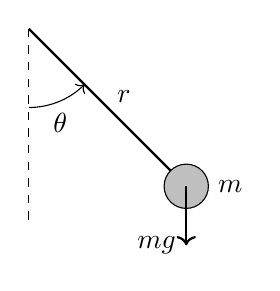
\begin{tikzpicture}
		\coordinate (O) at (0,0);
		\coordinate (P) at (2,-2);
		\draw[dashed] (O) -- ++(0,-2.5);
		
		\draw[thick] (O) -- (P);
		\draw[->] (O) -- node[midway, right, yshift=4] {$r$} (P);
		\filldraw[fill=gray!50] (P) circle (8pt);
		\node at (P) [right, xshift=8] {$m$};
		\draw[->, thick] (P) -- ++(0,-0.75) node[left] {$mg$};
		
		\draw[->] (0,-1) arc[start angle=-90,end angle=-45,radius=1];
		\node at (0.4,-1.2) {$\theta$};
	\end{tikzpicture}
}}
We want to find the relationship between the period, $\tau$ and $\theta,m,r$ and $g$. I.e. we want to find 
$$\tau = f(r, m, \theta, g)$$
First, lets find the dimensions of the system.
\begin{center}
	\begin{tabular}{|c|c|c|c|c|}
		\hline
		$[\tau]$ & $[r]$ & $[m]$ & $[\theta]$ & $[g]$ \\ \hline 
		$T$ & $L$ & $M$ & $1$ & $LT^{-2}$ \\ \hline
	\end{tabular}
\end{center}
\nt{$g$ is a dimensionless variable! In other words, its dimensions are $M^0L^0T^0$.\\}

The product of these varaibles takes the form:
$$
\tau^a r^b m^c \theta^d g^e
$$
and its dimensions are
$$
[\tau^a r^b m^c \theta^d g^e] = [\tau^a] [r^b] [m^c] [\theta^d] [g^e] = T^a\cd L^b \cd M^c \cd 1^d \cd L^eT^{-2e} = M^cL^{b+e}T^{a-2e}.
$$
Since we desire to solve represent a physical law, by claim 1.1.1, we know we're looking for a dimensionally homogeneous system.
\begin{align*}
	\Let M^cL^{b+e}T^{a-2e} &= M^0L^0T^0 \\
	\Then \left.\begin{array}{rcc}
		a - 2e & = & 0 \\
		b + e & = & 0 \\
		c & = & 0 
	\end{array}\right\rbrace& e = \frac{a}{2}, b = -\frac{a}{2}, d \text{ is free.}\\
\intertext{In other words, solve the linear system $A\utilde{x}=\utilde{0}$ (In other OTHER words, solve for the nullspace of $\cln(A)$.)}
	\tau^{a}r^{-\frac{a}{2}}m^0\theta^dg^{\frac{a}{2}} &= \bracks{\tau r^{-\half} g^\half}^a\theta^d \\
		&= \bracks{\tau\sqrt{\frac{g}{r}}}^a\theta^d
\intertext{By setting $(a,d)$ to $(1,0)$, and $(0,1)$, we obtain independent dimensionless products, $\Pi_1$ and $\Pi_2$.}
	\Pi_1 &= \tau\sqrt{\frac{g}{r}} \\
	\Pi_2 &= \theta
\end{align*}

\subsection*{The Buckingham $\Pi$-Theorem}
\thm{Buckingham $\Pi$-Theorem}{
	An equation is dimensionally homogeneous if and only if it can be written in the form
	$$
		f(\Pi_1, \Pi_2, \dots, \Pi_n) = 0,
	$$
	where $f$ is some function satisfying certain conditions (outside out scope) and $\braces{\Pi_1, \Pi_2, \dots, \Pi_n}$ is a complete set of dimensionless products corresponding to some mathematical model.
}

\nt{
	$\Pi_k$ is dimensionless, i.e.
	$\displaystyle
		\forall \Pi_k, [\Pi_k] = 1 
	$
}

The set $\bracks{\Pi_k}$ can be obtained by giving all solutions to a linear system of exponents for the model. We've found the complete set of dimensionless products for the pendulum problem, $\braces{\tau\sqrt{g/r}, \theta}$. Applying the Buckingham $\Pi$-theorem now, our mathematical model is of the form:
$$
	f(\Pi_1, \Pi_2) = 0 \implies f(\tau\sqrt{g/r}, \theta) = 0
$$
We further assume that from $f$ we can deduce 
\begin{gather*}
	\tau\sqrt{\frac{g}{r}} = h(\theta)\qquad \text{ by Implict Function Theorem.}
\end{gather*}
We'll describe implicit function theorem in detail later.

\nt{
	If $\Pi = \braces{\Pi_1, \Pi_2, \Pi_3}$, then $\Pi_1 = h(\Pi_1, \Pi_2)$. More generally, if $\Pi = \braces{\Pi_k\suchthat k\in\bbn,k\leq n}$, then $\Pi_1 = h\bracks{\Pi_2, \Pi_3, \dots, \Pi_n}$.
}

\subsection*{Archimedes' Law}
The famous ``Eureka!'' leaping from the bathtub one ;P\\

Archimedes' law applies to bodies immersed in a fluid. Consider a box of mass $m$, which displaces $V$ fluid, with constant density $\rho$. Suppose your class mate claims that this phenomenon is described by the equation
$$
	m\dyd[^2x]{t^2} = mg - mVg
$$
Let's verify this\dots
\begin{align*}
	\sqbracks{mVg} &= [m][V][g] \\
		&= M\cd L^3 \cd LT^{-2} \\
		&= ML^4T^{-2} \\
	\sqbracks{m\dyd[^2x]{t^2}} &= [m]\sqbracks{\dyd[^2x]{t^2}} \\
		&= MLT^{-2} \\
		&\neq [mVg]
\end{align*}
So we can conclude that this model is not dimensionally consistent.\\
Another classmate suggests the equation
$$
	m\dyd[^2x]{t^2} = mb - \rho Vg.
$$
We'll similarlly analyse this like
\begin{align*}
	\sqbracks{\rho Vg} &= [\rho][V][g] \\
		&= ML^{-3}\cd L^3 \cd LT^{-2} \\
		&= ML^1T^{-2} \\
		&= MLT^{-2} \\
\sqbracks{m\dyd[^2x]{t^2}} &= [m]\sqbracks{\dyd[^2x]{t^2}} \\
		&= MLT^{-2} \\
		&= \sqbracks{\rho Vg}
\end{align*}
Which is dimensionally consistent!\\

Let's use Buckingham $\Pi$-theorem to establish the general form any correct model must take:
\begin{gather*}
	\intertext{Consider the product $F^a\rho^bg^cV^dm^e$} 
	\begin{aligned}
		\sqbracks{F^a\rho^bg^cV^dm^e} &= (MLT^{-2})^a(ML^{-3})^b(LT^{-2})^c(L^3)^d(M)^e \\
			&= M^aL^aT^{-2a}\cd M^bL^{-3b}\cd L^cT^{-2c}\cd L^{3d}\cd M^e \\
			&= M^{a+b+e}L^{a-3b+c+3d}T^{-2a-2c} \\
		\Let M^0L^0T^0 &= M^{a+b+e}L^{a-3b+c+3d}T^{-2a-2c}
	\end{aligned} \\
	\Rightarrow\left.\begin{array}{rcc}
		a + b + e & = & 0 \\
		a - 3b + c + 3d & = & 0 \\
		-2a - 2c & = & 0
	\end{array}\right\rbrace\begin{array}{ccl}
		c & = & -a \\
		b & = & -a-e \\
		d & = & -a-e
	\end{array}\\
	\begin{aligned}
		\So F^a\rho^bg^cV^dm^e &= F^a\rho^{-a-e}g^{-a}V^{-a-e}m^e \\
			&= F^a\rho^{-a}g^{-a}V^{-a}\rho^{-e}V^{-e}m^e \\
			&= \bracks{F\rho^{-1}g^{-1}V^{-1}}^a \bracks{\rho^{-1}V^{-1}m}^e \\
			&= \bracks{\frac{F}{\rho gV}}^a \bracks{\frac{m}{\rho V}}^e \\
		\tf \Pi &= \braces{\frac{F}{\rho gV}, \frac{m}{\rho V}}.
	\end{aligned}
\end{gather*}

Now that we've deduced $\Pi$, we know that any valid physcial law must take the form:
$$
	\frac{F}{\rho gV} = h\bracks{\frac{m}{\rho V}}
$$
$$
	\implies F = \rho gV h\bracks{\frac{m}{\rho V}}
$$

\nt{
	Generally, when proceeding with the linear algebra portion of this procedure, keep in mind the power of your desired dependent variable, and try to express all other powers in terms of it. For example, in the pendulum example, and in the Archimedes' law exmaple too, we expressed the other variables in terms of $a$, because this was the power of the desired dependent variables $\tau$ and $F$, respectively. 
}

\section{Lecture 3}
\subsection*{Drag Force}
Consider a sphere of radius $r$, moving through a viscous fluidd. We wish to model the drag force, $F$, dependent on the relevant variables $\eta$, the viscosity, $v$, the velocity, and $r$ the radius.
\begin{gather*}
	\intertext{Consider the product $F^a\eta^bv^cr^d$} 
	\begin{aligned}
		[F]^a[\eta]^b[v]^c[r]^d &= \bracks{MLT^{-2}}^a\bracks{ML^{-1} T^{-1}}^b\bracks{LT^{-1}}^c\bracks{L}^d \\
			&= \bracks{M^aL^aT^{-2a}}\bracks{M^bL^{-b}T^{-b}}\bracks{L^cT^{-c}}\bracks{L^d} \\
			&= M^{a+b}L^{a-b+c+d}T^{-2a-b-c} \\
		\Let M^0L^0T^0 &= M^{a+b}L^{a-b+c+d}T^{-2a-b-c}
	\end{aligned}\\
	\Rightarrow \left.\begin{array}{rcc}
		a + b & = & 0 \\
		a - b + c + d & = & 0 \\
		-2a - b - c & = & 0
	\end{array}\right\rbrace \begin{array}{ccl}
		b & = & -a \\
		c & = & -a \\
 		d & = & -a
	\end{array} \\
	\begin{aligned}
		\So F^a\eta^bv^cr^d &= F^a\eta^{-a}v^{-a}r^{-a} \\
			&= \bracks{F\eta^{-1}v^{-1}r^{-1}}^{a} \\
			&= \bracks{\frac{F}{\eta v r }}^{a} \\
		\tf \Pi &= \braces{\frac{F}{\eta v r }}
	\end{aligned}
\end{gather*}
So from the Buckingham $\Pi$-theorem, we know that many valid physcial law must take the form:
$$
	f\bracks{\frac{F}{\eta vr}} = 0
$$
$$
	\implies \frac{F}{\eta vr} = k
$$
In other words, $F = k\eta vr$, where $k$ is some dimensionless constant.

\nt{
	This result, that drag force is proportional to velocity is known as Stokes' Law, and in fact, the constant $k=6\pi$.
}

\subsection*{A Mixing Model}
Initially, a tank of water with $v_0$ litres has $m_0$ grams of salt dissolved in it. Brine with $n$ grams of salt per litre runs into the tank at a rate of $x$ litres per minute. The contents are constantly stirred (so you can assume that the concentration of salt is always uniform throughout the tank) and water runs out of the tank at the rate of $y$ litres per minute. Let $s(t)$ denote the amount of salt in the tank at time $t$ (measured in minutes). Determine the equation which governs the net rate of change of salt, checking that all terms are dimensionally consistent.
\begin{gather*}
	\longintertext{Let $c(t)$ denote the density of salt at time $t$.\\
	Let $v(t)$ denote the volume of water in the tank at time $t$.}
	\begin{aligned}
		\text{We have } c(t) &=\frac{s(t)}{v(t)} \\
		\text{And } v(t) &= v_0 + (x-y)t \\
		\implies c(t) &= \frac{s(t)}{v_0+(x-y)t}. \\
	\end{aligned}
	\intertext{Salt enters at a rate of $nx$ grams/minute and leaves at a rate of $yc(t)$ per minute.}
	yc(t) = \frac{ys(t)}{v_0+(x-y)t}.
	\intertext{Therefore, the net rate of change is}
	\dyd[s]{t} = nx - \frac{ys}{v_0+(x-y)t}, s(0)=m_0.
	\intertext{Now lets check the model for dimensional homogeneity!}
	\begin{aligned}
		\sqbracks{\dyd[s]{t}} &= MT^{-1} \\
		[nx] &= ML^{-3}\cd L^3T^{-1} \\
			&= MT^{-1} \\
		[v_0] &= L^3 \\
		[(x-y)t] &= L^3T^{-1}T \\
			&= L^3 \\
		\Rightarrow \sqbracks{\frac{ys}{v_0+(x-y)t}} &= \frac{ML^3T^{-1}}{L^3} \\
			&= \frac{ML^3T^{-1}}{L^3} \\
			&= MT^{-1}
		\end{aligned}\\
		\tf \sqbracks{\dyd[s]{t}} = \sqbracks{nx} = \sqbracks{\frac{ys}{v_0+(x-y)t}}
\end{gather*}
So, the system is dimensionally homogeneous.

\subsection*{Scaling}
\textbf{Question,} can we scale experiments in a laboratory to ensure that the observed effects are consistent?\\
We can use dimensionless variables, and try to preserve their values. Some examples of dimensionless variables in fluid dynamics include
\begin{gather*}
	\text{Reynold's Number,}\qquad Re = \frac{\rho lv}{\eta} \\
	\text{Froude's Number,}\qquad Fr = \frac{v}{\sqrt{gl}} \\
	\text{Mach Number,}\qquad M = \frac{v}{c}
\end{gather*}
where, $\rho$ is the fluid denisty, $l$ is the length of an object, $v$ is velocty, $\eta$ is the viscosity of the fluid, $g$ is gravitational acceleration, and $c$ is the speed of sound.

\subsection*{A Ship Model}
Suppose our model involves $Fr$, which we seek to keep fixed. \\
The true boat has hull length $l=20\text{m}$, at speed $v=10\text{ms}^{-1}$\\
We can model this with a boat of hull length $l^*=0.2m$, i.e. $l^*=l/100$. \\
What is $v^*$?
\begin{gather*}
	\begin{aligned}
		Fr &= \frac{v}{\sqrt{gl}} = \frac{v^*}{\sqrt{gl^*}} \\
		\tf v^* &= v \sqrt{\frac{gl^*}{gl}} \\
			&= v \sqrt{\frac{l^*}{l}} \\
			&= 10 \sqrt{\frac{0.2}{20}} \\
		\tf v^* &= 1 \text{ms}^{-1}
	\end{aligned}
\end{gather*}

\chapter{Week 2}
\section{Lecture 4}
\subsection*{Multivariate Limits}
\subsubsection*{Review of one-variable case}
Let $f:\rmd\to\bbr$ be a function with domain $\rmd$, an open subset of $\bbr$. For $a\in\rmd$ we say that the limit $\dps{\lim_{x\to a}f(x)}$ exists if and only if (i) the left-sided limit exist, (ii) the right-sided limit exists, and (iii) these limits equal each other, namely
$$
	\lim_{x\to a^-} f(x) = \lim_{x\to a^+} f(x).
$$
Furthermore, if the limit exists, and is equal to the value of the function at $f$, namely,
$$
	\lim_{x\to a^-} f(x) = \lim_{x\to a^+} f(x) = f(a),
$$
we say that $f$ is continuous at $a$. The precise defintion of the one variable limit its
$$
	\lim_{x\to a}f(x)=L\iff \forall\veps>0,\exists\delta>0:0<\abs{x-a}<\delta\implies\abs{f(x)-L}<\veps.
$$
\subsubsection*{The two-variable case}
When $f$ is multivariate, finding the limit is more subtle. There are more then two ways to approach a given point. Consider 
$$
	f(x,y) = \frac{x^2}{x^2+y^2},
$$
with domain $\bbr^2\setminus{(0,0)}$.
We could approach this limit along the line $y=0$. If $x\neq0$,
\begin{gather*}
	f(x,0) = \frac{x^2}{x^2 + 0} = 1, \\
	\Then \lim_{x\to0} f(x,0) = \lim_{x\to0} 1 = 1
\end{gather*}
Suppose next we approach the limit along the line $x=0$, if $y\neq0$,
\begin{gather*}
	f(0,y) = \frac{0^2}{0^2 + y^2} = 0, \\
	\Then \lim_{y\to0} f(0,y) = \lim_{y\to0} 0 = 0.
\end{gather*}
Since we've approached the same point with two different paths, but found different limits,
$$
	\lim_{x\to0} f(x,0) \neq \lim_{y\to0} f(0,y),
$$
we can conclude that
$$
	\lim_{(x,y)\to(0,0)}f(x,y) \text{ does no exist.}
$$
For the limit $\dps{\lim_{(x,y)\to(a,b)} f(x,y)}$ to exist, it is necessary that \textit{every} path in $\rmd$ approaching $(a,b)$ gives the same limiting value. This presents us with a simple test for determining if a limit does not exist.

\ex{Test for showing no limit exists}{
	$$
		\text{If}\left\lbrace\begin{array}{rl}
			f(x,y)\to L_1 & \text{as } (x,y) \to (a,b) \text{ along the path } C_1\in\rmd \\
			f(x,y)\to L_2 & \text{as } (x,y) \to (a,b) \text{ along the path } C_2\in\rmd 
		\end{array}\right.
	$$
	such that $L_1\neq L_2$ then the limit $\dps{\lim_{(x,y)\to(0,0)}f(x)}$ does not exist.
}
\nt{
	The above notation is somewhat deficient and perhaps one shoule write
	$$
		\lim_{(x,y)\to_\rmd(a,b)}f(x,y)
	$$
	to indicate that only paths in $\rmd$ terminating at $(a,b)$ (which itself may or may not be in $\rmd$) are considered.
}
\qs{}{
	Let $\rmd=\bbr^2\setminus{(0,0)}$ and $f:\rmd\to\bbr$ be given by $\dps{f(x,y)\frac{x^2-y^2}{x^2+y^2}.}$ Show that the limit $\dps{\lim_{(x,y)\to(0,0)}f(x)}$ does not exist.
}
\sol Consider the path $C_1\in\rmd,y=0$ \\ If $x\neq0$,
\begin{gather*}
	f(x,0) = \frac{x^2}{x^2} = 1. \\
	\lim_{x\to0}f(x,0) = \lim_{x\to0}1 = 1.
	\longintertext{Consider the path $C_2\in\rmd,x=0$\\If $y\neq0,$}
	f(0,y) = \frac{-y^2}{y^2} = -1. \\
	\lim_{y\to0}f(0,y) = \lim_{y\to0}-1 = -1 \neq \lim_{x\to0}f(x,0). \\
	\intertext{Therefore, the limit $\dps{\lim_{(x,y)\to(0,0)}f(x,y)}$ does not exist.}
\end{gather*}

\qs{}{
	With the same $\rmd$ as the previous question, consider $\dps{f(x,y)=\frac{xy}{x^2+y^2}}$. Show that the limit $\dps{\lim_{(x,y)\to(0,0)}f(x,y)}$ does not exist.
}
\sol Consider the path $C_1\in\rmd,y=0$ \\ If $x\neq0$,
\begin{gather*}
	f(x,0) = 0 \implies \lim_{x\to0} f(x,0) = 0 \\
	\longintertext{Consider the path $c_2\in\rmd,x=0$\\ If $y\neq0$,}
	f(0,y) = 0 \implies \lim_{y\to0} f(0,y) = 0 \\
	\longintertext{Huh\dots I really thought that would work\dots\\Well, ok, Let's consider the path $C_3\in\rmd,x=y$\\ If $x\neq0$,}
	f(x,x) = \frac{x^2}{x^2+x^2} = \frac{1}{2} \implies \lim_{x\to0} f(x,x) = \frac{1}{2}.
	\intertext{Since this limit is different from the other two, we can conclude that the limit $\dps{\lim_{(x,y)\to(0,0)}f(x,y)}$ does not exist.}
\end{gather*}
\nt{
	We can look at finitely many paths, and easily show that a limit doesn't exisit, if two paths terminating at the same point have different limiting values. But, there are infinitely many paths in $\bbr^2$ which terminate at the point $(a,b)$. This raises the question, how can we prove a limit exists?
}

\noindent Consider the example 
$$
	\lim_{(x,y)\to(0,0)} f(x,y) = 0, \text{ where } f(x,y) = \frac{3x^2y}{x^2 + y^2} \text{ and } \rmd=\bbr\setminus{(0,0)}.
$$
We can argue that the above limit is correct and true by utilising a change of variables, namely $$x=r\cos\theta \qquad y=r\sin\theta$$
\sol
\begin{gather*}
	\begin{aligned}
			f(x,y) &= f(r\cos\theta,r\sin\theta) \\
				&= \frac{3r^2\cos^2\theta r\sin\theta}{r^2\cos^2\theta + r^2\sin^2\theta} \\
				&= \frac{3r^3\cos^2\theta\sin\theta}{r^2\bracks{\cos^2\theta +\sin^2\theta}} \\
				&= 3r\cos^2\theta\sin\theta
			\abs{\cos\theta} &\leq 1\\ 
			\abs{\sin\theta} &\leq 1 \\
			\implies \abs{\cos^2\theta\sin\theta} &\leq 1 \\
			\implies \abs{3r\cos^2\theta\sin\theta} &\leq 3r \\
			\implies \abs{f(x,y)} &\leq 3r 
	\end{aligned} \\
	\tf \text{as } r\to0, f(x,y)\to 0
\end{gather*}
No matter what path of form $(r,\theta)$ we take, as that path approaches the point $(a,b)$, the limit of $f(x,y)$ approaches 0. So we can argue that $\dps{\lim_{(x,y)\to(0,0)}f(x,y)}$ exists and is equal to 0. With everything we've learned now, let's finally, formally, define the limit of a multivariate function.

\dfn{The Limit of a Multivariate Function}{
	Let $f$ be a function of two variables, whose domain $\rmd$ includes points arbitrarily close to $(a,b)$. Then we say that the limit of $f(x,y)$ as $(x,y)$ approaches $(a,b)$ is $L$, written
	$$
		\lim_{(x,y)\to(a,b)} f(x,y) = L,
	$$
	if
	$$
		\forall\veps>0,\exists\delta>0:0<\sqrt{\bracks{x-a}^2 + \bracks{y-b}^2}<\delta\implies \abs{f(x,y)-L}<\veps.
	$$
}

\section{Lecture 5}
\subsection*{Multivariate Continuity}
\dfn{Multivariate Continuity}{
	Given a function $f:\rmd\to\bbr$, where $\rmd$ is an open subset of $\bbr^2$. Let $(a,b)\in\rmd$. Then $f(x,y)$ is continuous at $(a,b)$ If
	$$
		\lim_{(x,y)\to(0,0)}f(x,y)=f(a,b),
	$$
	ie, the limit $(x,y)\to(a,b)$ of $f(x,y)$ exists and is equal to $f(a,b)$.\\
	
	Equivalently, $f$ is continuous if 
	$$
		\forall\veps>0,\exists\delta>0: (x,y)\in\rmd\land\sqrt{(x-a)^2+(y-b)^2}<\delta\implies\abs{f(x,y)}<\veps.
	$$
}
\nt{
	An open subset is a subset which does not have boundary points. As opposed to a closed subset which has boundary points. More formally, ``open'' $=$ for every point $p\in\rmd$, there is a disc with centre $p$ that lies entirely in $\rmd$. So, if you took $p$ on the bounary, you can never find a disc which is entirely inside $\rmd$, you'll always have a little bit peaking out of it.
}
\noindent So, is 
$$
	f(x,y) = \frac{x^2 - y^2}{x^2 + y^2}, \rmd=\bbr^2\setminus{(0,0)}
$$
continuous?\\
Well, even though we already found that this limit $(x,y)\to(0,0)$ does not exist, we note that $(0,0)\notin\rmd$. Therefore, it is continuous.\\
If we amend the domain to include $(0,0)$, the function is no longer continous, because the limit $(x,y)\to(0,0)$ does not exist.

\subsection*{Limit Laws}
Suppose $\dps{\lim_{(x,y)\to(a,b)}f(x,y)}$ and $\dps{\lim_{(x,y)\to(a,b)}g(x,y)}$ exist. \\
Below, for ease of notation, $\lim$ denotes $\dps{\lim_{(x,y)\to(a,b)}}$. \\
\begin{enumerate}
	\item $\lim(f(x,y)\pm g(x,y)) = \lim f(x,y) \pm\lim g(x,y)$.
	\item $\lim cf(x,y) = c\lim f(x,y)$, where $c$ is some constant. 
	\item $\lim(f(x,y)\cd g(x,y)) = \lim f(x,y) \cd \lim g(x,y)$.
	\item $\dps{\lim\frac{f(x,y)}{g(x,y)} = \frac{\lim f(x,y)}{\lim g(x,y)}}$, if $\lim g(x,y)\neq 0$.
\end{enumerate}

\section{Lecture 6}
\subsection*{Partial Derivatives}
\subsubsection*{Slope in the x-direction}
Consider the surface $z=f(x,y)=1-x^2-y^2$, and the point $P=(1,-1,-1)$. Holding $y$ constant, we can we can find a cross section of the surface at that point.
$$
	\Let g(x) = f(x,-1)=1-x^2-1 = -x^2
$$
We can find the slope tangent of the surface $z$ at the point $P$, in the x-direction, by differentiating $g(x)$,
$$
	g'(x) = -2x \implies g'(1) = -2
$$

\subsubsection*{Slope in the y-direction}
We can follow a similar procedure by holding $x$ constant, and generating the y-direction cross section of the surface $z$
$$
	\Let h(y) = f(1,y) = 1-1-y^2 = -y^2
$$
Now, we can evaluate the y-direction slope of the tanget of the surface $z$ at the point $P$ by taking the derivative of $h(x)$, namely
$$
	h'(x) = -2y \implies h'(-1) = 2.
$$

\subsubsection*{Another example}
Given $f(x,y)=xy^3 + x^2$, find $f_x(1,2)$ and $f_y(1,2)$.
\begin{gather*}
	\begin{aligned}
		f(x,y) &= xy^3 + x^2 \\
		\tf f_x(x,y) &= y^3 + 2x \\
		\implies f_x(1,2) &= 8 + 2 = 10 \\
		\tf f_y(x,y) &= 3xy^2 + 0 = 3xy^2 \\
		\implies f_y(1,2) &= 3\cd1\cd4 = 12 
	\end{aligned}
\end{gather*}
Nothing scary :)

\subsubsection*{Partial derivative for $f(x,y,z)$}
Consider the volume of a box, $V(x,y,z) = xyz$. If $x$ changes by an an amount, say $\Delta x$, the volume will change by some amount, $\Delta V$. One can visualise the change in volume, by imagine a box being concatonated to the original box, with width $\Delta x$, height $y$, and depth $z$. Therefore $\Delta V = yz\Delta x$. This leads us to see that
$$
	\frac{\Delta V}{\Delta x} = yz.
$$
Now, letting $\Delta x\to 0$, we can find $\dps{\frac{\partial V}{\partial x} = yz}$.\\
With partial derivatives, only one of the independent variables is allowed to change; all other variables are held constant.
$$
	\frac{\partial V}{\partial x} = \lim_{\Delta x \to 0} \frac{V(x+\Delta x, y, z) - V(x, y, z)}{\Delta x}
$$

\subsubsection*{Higher order derivatives}
\begin{multicols}{2}
	\noindent
	\begin{gather*}
		f_{xx} = \Del{2}{f}{x} \\
		f_{yy} = \Del{2}{f}{y} \\
		f_{xy} = \del{^2f}{x\partial y} = \del{}{y}\bracks{\del{f}{x}}\\
		f_{yx} = \del{^2f}{y\partial x} = \del{}{x}\bracks{\del{f}{y}}\\
	\end{gather*}
\end{multicols}
\thm{Clairaut's Theorem}{
	Suppose $f$ is defined on a disk $D$ that contains the point $(a,b)$. If the functions $f_{xy}$ and $f_{yx}$ are both continuous, then $f_{xy}(a,b) = f_{yx}(a,b)$.
}
\noindent By extension, if $f_{xy}$ and $f_{yx}$ are both continuous everywhere, then $f_{xy} = f_{yx}$.
\qs{}{
	Find all the first and second order derivatives of $f(x,y) = x\sin y + y\cos x$ and show that $f_{xy} = f_{yx}$.
}
\sol
\begin{gather*}
	\begin{aligned}
		f_x(x,y) &= \sin y - y\sin x \\
		f_y(x,y) &= x\cos y + \cos x \\
		f_{xx}(x,y)  &= -y\cos x \\
		f_{yy}(x,y) &= -x\sin y \\
		f_{xy}(x,y) &= \del{f_x}{y} \\
			&= \cos y - \sin x \\
		f_{yx}(x,y) &= \del{f_y}{x} \\
			&= 	\cos y - \sin x \\
		\tf f_{xy} &= f_{yx} 
	\end{aligned}
\end{gather*}

\noindent An unexpected feature of multivariate calculus is the possiblity that the for some point $P$, the partial derivatives of a function may be well defined, and yet, the function is not continuous at $P$. This is opposed to the one dimensional case, where we (na\"ively), assert that continuity $\implies$ differentiability. Consider 
$$
	f(x,y) = \left\lbrace\begin{array}{ll}
		\dfrac{xy}{x^2+y^2} & \text{for } (x,y)\neq(0,0) \\
		0 & \text{for } (x,y) = (0,0)
	\end{array}\right.
$$
The derivatives at $(0,0)$ are well defined:
$$
	\del{f}{x} = \frac{y^3 - x^2y}{(x^2+y^2)^2} \implies \del{f}{x}(0,0) = \lim_{h\to0} \frac{f(h, 0) - f(0,0)}{h} = \lim_{h\to 0} \frac{0 - 0}{h} = 0
$$
($\dps{\del{f}{y}}$ is defined and equal to $\dps{\del{f}{x}}$, because the function is symmetric, note that x and y can be simply interchanged in the function definition.)\\
Here, we have a function, whose derivatives are defined at a point $P$, and yet, is discontinuous at $P$.\\
When dealing with multivariate functions, existent derivatives are insufficient for determining differentiability.

\chapter{Week 3}
\section{Lecture 7}
\subsection*{The Tangent Plane}
Recall the one dimensional case, for a function $y=f(x)$, and a point $(a, f(a))$, the tangent line is given by
$$
	y_\top = f(a) + f'(a)(x-a)
$$
and can be derived by considering
\begin{gather*}
	y_\top = mx + c \\
	x = a\qquad y = f(a)\qquad m = f'(a) \\
	\tf f(a) = f'(a)a + c \\
	\tf c = f(a) - f'(a)a \\
	\tf y_\top = f'(a)x + f(a) - f'(a)a \\
	\tf y_\top = f(a) + f'(a)(x-a) 
\end{gather*}
Let's derive the vector equation for of a tangent line, consider the vector
$$
	\ut{r}(x) = (x, f(x)),
$$
and another vector which is some $\Delta x$ away from $\ut{r}$,
$$
	\ut{r}(x+\Delta x) = (x + \Delta x, f(x+\Delta x)).
$$
Now consider $\ut{r}(x+\Delta x) - \ut{r}(x) / \Delta x$. As we allow $\Delta x$ to go to 0, $\ut{r}(x+\Delta x) - \ut{r}(x)$ is going to approach the tangent line, of $f(x)$ at the point $(x,f(x))$.
$$
	\lim_{\Delta x\to 0}\frac{\ut{r}(x+\Delta x) - \ut{r}(x)}{\Delta x} = \lim_{\Delta x\to 0} \begin{pmatrix}
		\dfrac{x + \Delta x - x}{\Delta x} \\
		\dfrac{f(x+\Delta x) - f(x)}{\Delta x}
	\end{pmatrix} = \begin{pmatrix}
		1 \\ f'(x)
	\end{pmatrix}
$$
Therefore, the tangent vector, $\ut{r}_\top$ is $(1, f(x))$. Points on lying on the tangent, are 
$$
	\begin{pmatrix}
		x \\ y
	\end{pmatrix}
	=
	\begin{pmatrix}
		x_0 \\ y_0
	\end{pmatrix}
	+ 
	\lm \begin{pmatrix}
		1 \\ f'(x_0)
	\end{pmatrix},
$$
where $(x,y)$ is the point on the line, $(x_0, y_0)$ are the inital conditions, namely, the point lying on $f(x)$, and $\lambda$ is some real number. We went to all this effort, because the tangential plane of a 3D surface, is analogous to the tangential lin on a 2D curve.

\subsubsection*{Equation for the tagent plane}
On a surface $z=f(x,y)$, at the point $(a,b,f(a,b))$, the tangent plane is given by
$$
	\boxed{z_\top = f(a,b) + f_x(a,b)(x-a) + f_y(a,b)(y-b)}
$$
This is analogous to the 2D case. We follow this by defining the plane as a vector
$$
	\boxed{\ut{r}_\top = (r_1,r_2,r_3) = (a,b,f(a,b)) + \lm(1, 0, f_x(a,b)) + \mu(0, 1, f_y(a,b)),}
$$
where $\lm=x-a$ and $\mu=y-b$.\\

\noindent I like to think of it like this:
$$
	\ut{r}_x = (1, 0, f_x(a,b))\qquad \ut{r}_y = (1, 0, f_y(a,b))
$$
are linearly independent vectors. The $\Span\braces{\ut{r}_x, \ut{r}_y}$ \textit{is} the tangent plane. $\lm,\mu\in\bbr$ lets us take any linear combination of these planar basis vectors. This new vector, therefore, will lie on the tangent plane. 

\ex{Tangent Plane}{
	Find the tangent plane to the surface $z=1-x^2-y^2$ at the point $P=(1,-1,-1)$.
	\begin{gather*}
		\begin{aligned}
			f(x,y) &= 1 - x^2 - y^2 \implies f(1,-1) = -1 \\
			f_x(x,y) &= -2x \implies f_x(1,-1) = -2 \\
			f_y(x,y) &= -2y \implies f_y(1,-1) = 2 \\
			\tf z_\top &= -1 - 2(x-1) + 2(y+1) \\
				&= -1 -2x +2 +2y + 2 \\
				&= 3 - 2x + 2y 
		\end{aligned}
		\intertext{Alternatively\dots}
		\ut{r}_\top
		= 
		\begin{pmatrix}
			r_1 \\ r_2 \\ r_3
		\end{pmatrix}
		=
		\begin{pmatrix}
			1 \\ -1 \\ -1
		\end{pmatrix}
		+ 
		\lm\begin{pmatrix}
			1 \\ 0 \\ -2
		\end{pmatrix}
		+
		\mu\begin{pmatrix}
			0 \\ 1 \\ 2
		\end{pmatrix} 
		= 
		\begin{pmatrix}
			1 + x - 1 + 0 \\ -1 + 0 + y - 1 \\ -1 - 2x + 2 + 2y + 2
		\end{pmatrix}
		=
		\begin{pmatrix}
			x \\ y \\ 3 - 2x + 2y
		\end{pmatrix}
	\end{gather*}
}

\ex{Tangent Plane}{
	What is the plane tangent to the surface $f(x,y) = 4 - x^2 + 4x - y^2$, at $(1,1)$?
	\begin{gather*}
		\begin{aligned}
			f(1,1) &= 4 - 1 + 4 - 1 = 6 \\
			f_x(x,y) &= -2x + 4 \implies f_x(1,1) = 2 \\
			f_y(x,y) &= -2y \implies f_y(1,1) = -2 \\
			\tf z_\top(x,y) &= 6 + 2(x-1) - 2(y-1) \\
				&= 6 + 2x - 2 - 2y + 2 \\
				&= 6 + 2x - 2y
		\end{aligned}
	\intertext{Alternatively\dots}
	\ut{r}_\top 
	=
	\begin{pmatrix}
		r_1 \\ r_2 \\ r_3
	\end{pmatrix}
	=
	\begin{pmatrix}
		1 \\ 1 \\ 6
	\end{pmatrix}
	+
	\lm\begin{pmatrix}
		1 \\ 0 \\ 2
	\end{pmatrix}
	+
	\mu\begin{pmatrix}
		0 \\ 1 \\ -2
	\end{pmatrix}
	=
	\begin{pmatrix}
		1 + x - 1 + 0 \\ 1 + 0 + y - 1 \\ 6 + 2x - 2 - 2y + 2
	\end{pmatrix}
	=
	\begin{pmatrix}
		x \\ y \\ 6 + 2x - 2y
	\end{pmatrix}
	\end{gather*}
}

\subsubsection*{Smoothness}
A surface, $z = f(x,y)$ is smooth at a point $(a,b)$ if $f$, $f_x$ and $f_y$ are all continuous at $(a,b)$. Informally, as you zoom more and more into $(a,b)$, it looks more and more like a flat plane.\\
One way to observe this is looking at contours. As you zoom into a smooth function, the contours will straighten out. This means that, close to $(a,b)$, the surface can be approximated with a plane; in fact, approximated with the tangent plane.\\
Examples of non-smooth functions include things like Brownian motion. No matter how much you zoom into Brownian motion, it always looks rough. In fact, Brownian motion is fractal.

\section{Lecture 8}
We first note, that the first order approximation of a single variable function, $f(x)$, around some point $(a, f(x))$, is a straight line tanget to that point.
$$
	f(a)\approx f(a) + f'(a)(x-a)
$$
\ex{}{
	Given $f(x)=\exp(x)$, estimate $e^{0.1}$.
	\begin{gather*}
		f(x) = \exp(x) \implies f'(x) = \exp(x) \\
		f(0) = \exp(0) = 1 \implies f'(0) = \exp(0) = 1 \\
		\tf e^{0.1} \approx f(0) + f'(0)(x-0) \\
		e^{0.1} \approx 1 + x \\
		\tf e^{0.1} \approx 1.1
	\end{gather*}
}

\subsection*{Linear Approximations for $f(x,y)$}
The corresponding linear, or first order approximation for a function $f$, of two variables, near a known point $(a,b)$, is the tangent plane centred on that point, given that $f$ is a smooth. Therefore, the approximation of $f$ at $(a,b)$ is
$$
	f(x,y)\approx f(a,b) + f_x(x,y)(x-a) + f_y(x,y)(y-b)
$$
\ex{}{
	The temperature in a region is given by $T(x) = 100 - x^2 - y^2$. Find the linear approximation to $T(x,y)$ near $(0,5)$.
	\begin{gather*}
		T(x,y) = 100 - x^2 - y^2 \implies T(0,5) = 75 \\
		T_x(x,y) = -2x \implies T_x(0,5) = 0 \\
		T_y(x,y) = -2y \implies T_y(0,5) = -10 \\
		\tf T(x,y) \approx T(0,5) + T_x(0,5)(x-0) + T_y(0,5)(y-5) \\
		T(x,y) \approx 75 + 0 + (-10)(y-5) \\
		T(x,y) \approx 125 - 10y 
	\end{gather*}
}

\ex{}{
	Find the tangent plane to $z=\exp(-x^2)\sin y$ at $(1, \pi/2)$. Use it to approximate $e^{-(0.9)^2}\sin(1.5)$.
	\begin{gather*}
		\intertext{Note: 0.9 is close to 1, and 1.5 is close to $\pi/2$.}
		f(x,y) = \exp(-x^2)\sin y \implies f(1, \pi/2) = \exp(-1) \\
		f_x(x,y) = -2x\exp(-x^2)\sin y \implies f_x(1,\pi/2) = -2\exp(-1) \\
		f_y(x,y) = \exp(-x^2)\cos y \implies f_y(1,\pi/2) = 0 \\
		z \approx f(1,\pi/2) + f_x(1,\pi/2)(x-1) + f_y(1, \pi/2)(y-\pi/2) \\
		\implies z \approx \exp(-1)(3-2x) \\
		\tf e^{-0.9^2}\sin(1.5) \approx e^{-1}\bracks{3-2\cd 0.9} \approx 0.4415
	\end{gather*}
}

\subsection*{Differentials}
If we reduce small changes $\Delta x$ and $\Delta y$ down to an infinitesimal changes, $\d x$, $\d y$, the linear approximation as
$$
	\d z = \d f = f_x(a,b)dx + f_y(a,b)dy
$$
This infinitesimal change $dz$ is called the total differential, and is definied by this equation (note the ``='', instead of an ``$\approx$'').

\begin{gather*}
	\intertext{Consider the work done by a, $W=PV$, where $P$ is pressure and $V$ is volume.}
	W(P,V) = PV \\
	W(P+\D P, V+\D V) = (P+\D P)(V+\D V) = PV + P\D V + V\D V + \D P\D V \\
	\tf \D W = P\D V + V\D V + \D P\D V \\
	\Let \d P = \D P, \text{ as }\D P\to 0, \d V = \D V, \text{ as }\D V\to 0 \\
	\tf \d W = P\d V + V\d V ( = W_P(P,V)\d P + W_V(P,V)\d V)
	\text{Note: } \D P\D V = 0
\end{gather*}

\subsection*{Estimating Error}
If the error in $x$ and $y$ is, at most$E_x$, and $E_y$, respectively, then a resaonable estimate for the worst-case error in the linear approximation of $f$ at $(a,b)$ is
$$
	|E| \approx |f_x(a,b)E_x| + |f_y(a,b)E_y|
$$

\ex{}{
	Suppose when making a metal barrel of base radius 1m, and height 2m, we allow an error of 5\% in radius and height. Estimate the worst-case error in volume.
	\begin{gather*}
		V(r,h) = \pi rh^2 \implies V_r(r,h) = 2\pi rh, V_h(r,h) = \pi r^2 \\
		\tf V(1,2) = 2\pi, V_r(1,2) = 4\pi, V_h(1,2) = \pi \\
		E_r = \frac{5}{100}r = \frac{5}{100}(1) = 0.05 \\
		E_h = \frac{5}{100}h = \frac{5}{100}(2) = 0.1 \\
		\implies |E| = |V_r(1,2)E_r| + |V_h(1,2)E_h| = \abs{4\pi \cd \frac{5}{100}} + \abs{\pi \cd \frac{10}{100}} = \frac{3\pi}{10} \\
		\implies\text{pct\% error: }\frac{|E|}{V(1,2)}\cd100 = \frac{3\pi}{10\cd2\pi}\cd100 = 15\%
		\intertext{Therefore, an estimate for the worst-case error in volume is 15\%}
	\end{gather*}
}
\nt{
	$\d V = V_r(1,2)\d r + v_h(1,2)\d h$, and $\d r = \D r = E_r$, $\d h = \D h = E_h$. \\
	$|E| = |V_r(1,2)E_r| + |V_h(1,2)E_h$. \\
	So the error in $V$ is just the differential of $V$.
}

\section{Lecture 9}
\subsection*{Differentiability}
Recall that in single variable calculus, a function $f$ is differentiable at $x_0$ if there exists a number $f'(x_0)$ such that
$$
	f'(x_0) = \lim_{h\to0} \frac{f(x_0 + h) - f(x_0)}{h} 
$$
which can be rewritten as 
$$
	0 = \lim_{h\to0} \frac{f(x_0 + h) - f(x_0) - f'(x_0)h}{h}
$$
Informally, we say $f$ is differentiable at $x_0$ if, after enough zooming, we see a stright line $y(x) = f(x_0)+f'(x_0)(x-x_0)$, such that the difference $f(x_0+h) - y(x_0+h)$ goes to 0, faster then linearly in the limit as $h$ goes to 0. \\

Extending to the multivariate case, let $V\subseteq \bbr^n$. We define a function $f:V\to\bbr$ to be differentiable at $\ut{a}$ if there exists $\grad f(\ut{a})\in\bbr^n$ such that 
$$
	\lim_{\ut{h}\to \ut{0}} \frac{f(\ut{a}+\ut{h}) - f(\ut{a}) - \grad f(\ut{a})\cd\ut{h}}{||\ut{h}||} = 0
$$
Informally, we say that $f$ is differentiable at $\ut{a}$, if there is a plane $z(\ut{a}+\ut{h}) = f(\ut{a}) + \grad f(\ut{a})\cd\ut{h}$ such that $f(\ut{a}+\ut{h}) - z(\ut{a}+\ut{h})$ goes to 0 faster then linearly as $\ut{h}$ goes to $\ut{0}$. \\

As we shall see, if it is possible for a tangent plane, $z$ to exisit at the point $\ut{a}$, but for the function $f:V\to\bbr$ to not be differentiable at that point. \\

The lecturer proceeded to give us a very nice geometric interpretation of this, but I'm not going to write everything he handwrote.

\thm{}{
	If a function is differentiable at a point, then it is continuous at that point. The contrapositive of this is, if a function is not continuous at a point, then it is not differentiable at that point.
}

\thm{}{
	If all first-order partial derivatives of a function exist and are continuous at a point, then the function is differentiable at that point.
}

\chapter{Week 4}
\section{Lecture 10}
\subsection*{Gradients and Directional Derivatives}
The partial derivative $f_x$ corresponds to the slope of $f(x,y)$ in the $x$-direction. We now turn out attention to the question of slopes in arbitrary directions, such as $\ihat + 2\jhat$ or $-\jhat$. \\

Let $\ut{u}=\bracks{u_1,u_2,\dots,u_n} \in\bbr^n:||\ut{u}||=1$. The directional derivative of $f$ at the point $\ut{a}$ in the direction $\ut{u}$ be defined as:
$$
	f_{\ut{u}}(\ut{a})\equiv \lim_{t\to0} \frac{f(\ut{a} + t\ut{u}) - f(\ut{a})}{t}.
$$
It is also known as the slope of $f$ at the point $\ut{a}$ in the direction of $\ut{u}$. \\

In practice, this is quite cumbersome though. Instead, if $f$ is differentiable, we can observe that
\begin{gather*}
	\lim_{h\to0}\frac{f(\ut{a}+\ut{h}) - f(\ut{a}) - \grad f(\ut{a})\cd\ut{h}}{||\ut{h}||} = \lim_{t\to0}\frac{f(\ut{a}+t\ut{u}) - f(\ut{a}) - \grad f(\ut{a})\cd t\ut{a}}{t} = 0 \\
	\intertext{We can then write}
	\begin{align*}
		f_{\ut{u}} &= \lim_{t\to0}\frac{f(\ut{a}+t\ut{u}) - f(\ut{a})}{t} + \grad f(\ut{a})\cd \ut{u} - \grad f(\ut{a})\cd \ut{u} \\
			&= \lim_{t\to0}\frac{f(\ut{a}+t\ut{u}) - f(\ut{a}) - \grad f(\ut{a})\cd t\ut{u}}{t} + \grad f(\ut{a})\cd \ut{u}  \\
			&= \lim_{t\to0}\frac{f(\ut{a}+t\ut{u}) - f(\ut{a}) - \grad f(\ut{a})\cd t\ut{u}}{t} + \lim_{t\to0} \grad f(\ut{a})\cd \ut{u}  \\
			&= 0 + \lim_{t\to0} \grad f(\ut{a})\cd \ut{u} \\
			\Aboxed{f_{\ut{u}} &= \grad f(\ut{a})\cd \ut{u}}  
	\end{align*}
\end{gather*}
We can drop our assumption that $\ut{u}$ is a unit vector, and instead write 
$$
	f_{\ut{u}} = \grad f(\ut{a}) \cd \frac{\ut{u}}{||\ut{u}||}
$$

\subsection*{The gradient vector $\grad f$}
The gradient vector of $f$, or the gradient of $f$ is the simply the vector whose components are partial derivatives. \\

If we let $\braces{\ut{b}_1, \ut{b}_2, \dots, \ut{b}_n}$ form the canonical basis of $\bbr^n$ then,
$$
	\grad \in\bbr^n: \grad = \sum_{i=1}^{n} \ut{b_i}\del{}{x_i},
$$
where $x_i$ is the $i$th Cartesian dimension, or $i$th component of a vector in $\bbr^n$. \\

For example in two dimensions
$$
	\mathop{\text{grad}} f = \grad f = (f_x, f_y) = f_x\ihat + f_y\jhat.
$$
But this totally generalises into higher dimensions, for example, for a four variable function, $f(x,y,z,w)$,
$$
	\mathop{\text{grad}}f = \grad f = (f_x, f_y, f_z, f_w) = f_x\ihat + f_y\jhat + f_z\khat + f_w\hat{l}
$$

\ex{}{
	If $f(x,y)=x^2 - 3y^2 + 6y$, find the slope at $(1,0)$ in the direction $\ihat - 4\jhat$.
	\begin{gather*}
		\grad f = \begin{pmatrix}
			f_x \\ f_y
		\end{pmatrix} = \begin{pmatrix}
			2x \\ 6 - 6y 
		\end{pmatrix} \implies 
		\grad f(1,0) = \begin{pmatrix}
			2 \\ 6
		\end{pmatrix} \\
		\ut{u} = \begin{pmatrix}
			1 \\ -4
		\end{pmatrix} \implies
		\hat{\ut{u}} = \frac{1}{\sqrt{1^2 + 4^2}}\begin{pmatrix}
			1 \\ -4
		\end{pmatrix} = \begin{pmatrix}
			1 / \sqrt{17} \\ -4 / \sqrt{17}
		\end{pmatrix} \\
		\implies f_{(1,-4)}(1,0) = \grad f(1,0) \cd \hat{\ut{u}} = \begin{pmatrix}
			1 \\ -4
		\end{pmatrix} \cd \begin{pmatrix}
			1/\sqrt{17} \\ -4/\sqrt{17}
		\end{pmatrix} = \frac{2}{\sqrt{17}} - \frac{24}{\sqrt{17}} = \frac{-22}{\sqrt{17}}
	\end{gather*}
}

\ex{}{
	Find $f_{(1,-1)}(0,1) \text{ for } f(x,y) = x - x^2y^2 + y$
	\begin{gather*}
		\grad f = \begin{pmatrix}
			f_x \\ f_y
		\end{pmatrix} = \begin{pmatrix}
			1 - 2xy^2 \\ 1 - 2x^2y
		\end{pmatrix} \implies \grad f(0,1) = \begin{pmatrix}
			1 \\ 1
		\end{pmatrix} \\
		\ut{u} = \begin{pmatrix}
			1 \\ -1
		\end{pmatrix} \implies \hat{\ut{u}} = \frac{1}{\sqrt{1^2 + 1^2}} \begin{pmatrix}
			1 \\ -1
		\end{pmatrix}  = \begin{pmatrix}
			1 / \sqrt{2} \\ -1/\sqrt{2}
		\end{pmatrix} \\
		\implies f_{(1,-1)}(0,1) = \grad f(0,1)\cd\hat{\ut{u}} = \begin{pmatrix}
			1 \\ 1
		\end{pmatrix} \cd \begin{pmatrix}
			1/\sqrt{2} \\ -1/\sqrt{2}
		\end{pmatrix} = \frac{1}{\sqrt{2}} - \frac{1}{\sqrt{2}} = 0
	\end{gather*}
}

\subsection*{Properties of the gradient vector}
Two important properties of the gradient vector are:\\

The gradient $\grad f(a,b)$ is perpendicular to the contour line through (a,b) and points in the direction of the greatest increase of $f$. In fact, the direction and magnitude of the steepest slope at $(a,b)$ are given by $\grad f(a,b)$ and $||\grad f(a,b)||$.\\

We can understand these two facts by considering the value of $\cos\theta$ in 
$$
	f_{\ut{u}} = \grad f \cd \frac{\ut{u}}{||\ut{u}||} = ||\grad f||\cos\theta
$$
Consider $\ut{A}\cd\ut{B} = ||\ut{A}||\ ||\ut{B}||\cos\theta$
\begin{itemize}
	\item Case 1. $\theta = 0$\\ $\grad f$ and $\ut{u}$ are in the same direction.\\ $f_{\ut{u}}$ is maximised, because $\cos0 = 1$.
	\item Case 2. $\theta = \pi$\\ $\grad f$ and $\ut{u}$ are in opposite directions.\\ $f_{\ut{u}}$ is minimised, because $\cos\pi = -1$.
	\item Case 3. $\theta = \frac{k\pi}{2}$\\ $\grad f$ and $\ut{u}$ are perpendicular to each other.\\ $f_{\ut{u}}$ is 0. We can conclude $f(x,y)=C$, the value of $f$ doesn't change, as we move along the contour.
\end{itemize}

\ex{}{
	$T(x,y)=20 - 4x^2 - y^2$ describes the temperature on the surface of a metal plate. In which direction away from the point $(2,-3)$ does the temperature change most rapidly? In which directions away from the point $(2,-3)$ is the temperature not change? 

	\begin{gather*}
		T(2,-3) = 20 - 4(2)^2 - (-3)^2 = 20 - 16 - 9 = -5\\
		\intertext{The point $(2,3)$ lies on a contour line, lets find that line,}
		-5 = T(2, -3) = 20 - 4x^2 - y^2 \implies 4x^2 + y^2 = 25 \text{ an ellipses.} \\
		\implies \grad T = \begin{pmatrix}
			-8x \\ -2y
		\end{pmatrix} \implies \grad T(2,-3) = \begin{pmatrix}
			-16 \\ 6
		\end{pmatrix}
		\intertext{$\implies$At $(2,3)$, temperature is most rapidly increasing in the direction of $(-16,6)$.}
		\text{Direction of no change} = \ut{u}: \grad T\cd\ut{u} = 0 \\
		\grad T(2,-3)\cd\ut{u} = \begin{pmatrix}
			-16 \\ 6
		\end{pmatrix} \cd \begin{pmatrix}
			u_1 \\ u_2
		\end{pmatrix} = -16u_1 + 6u_2 = 0 \\
		\tf \ut{u} \in \braces{\begin{pmatrix} 6 \\ 16 \end{pmatrix}, \begin{pmatrix} -6 \\ -16 \end{pmatrix}}
	\end{gather*}
}

\section{Lecture 11}
Let's go over the one variable case. If $y=f(u)$ and $u=g(x)$, then 
$$
	\dydx = \dyd{u}\dyd[u]{x} \qquad\text{or}\qquad y'(x) = f'(u)g'(x)
$$
\ex{}{
	A simple one first, what is $\dydx$ given $y = (x^2+5)^5$
	\begin{gather*}
		y = f(u) = u^5,\ u = g(x) = x^2+5,\qquad 
		\dydx = \dyd[f]{u}\cd\dyd[u]{x} = 5u^4\cd 2x = 10x(x^2+5)^4.
	\end{gather*}
}
\ex{}{
	Suppose the radius of a cylinder decreases at a rate of $r'(t)=-2$cm/s. How fast is the volume decreasing?
	\begin{gather*}
		V = \pi r^2h,\ \text{fix}\ h=2, \implies V(r) = 2\pi r^2 \\
		\dyd[r]{t}=-2,\ \dyd[V]{r}=4\pi r \\
		\dyd[V]{t} = \dyd[V]{r}\cd\dyd[r]{t} = 4\pi r\cd-2 = -8\pi r \\
		\tf \left.\dyd[V]{t}\right|_{r=1} = -8\pi\text{cm}^3/\text{sec}.
	\end{gather*}
}

\subsection*{The Multivariate Chain Rule}
Let $U\subseteq \bbr^n$ and $V\subseteq\bbr$, and $f:U\to\bbr$, $\ut{x}=(x_1,x_2,\dots,x_n)$ such that $x_i:V\to\bbr$, then, provided that $f$ and all $x_i$ are differentiable,
$$
	\left. \dyd{t} f(\ut{x}(t)) \right|_{t=t_0} = \sum_{i=1}^{n}\del{f(\ut{x}(t_0))}{x_i}x'_i(t_0)
$$
Daunting as it looks, it's really quite simple, let's take $n=2$ for example. Suppose $z=f(x,y)$ and $x$ and $y$ are both functions with respect to $t$. Then 
$$
	\dyd[z]{t} = \dyd[z]{x}\cd\dyd[x]{t} + \dyd[z]{y}\cd\dyd[y]{t}
$$
If we take $n=4$, $z=f(a,b,c,d)$,
$$
	\dyd[z]{t} = \dyd[z]{a}\dyd[a]{t} + \dyd[z]{b}\dyd[b]{t} + \dyd[z]{c}\dyd[c]{t} + \dyd[d]{a}\dyd[d]{t}
$$
\ex{}{
	Suppose $z = f(x, y) = 4x^2 + 3y^2$ and $x(t) = \sin t$, $y(t) = \cos t$. Then 
	\begin{gather*}
		\dyd[z]{x} = 8x,\qquad \dyd[x]{t} = \cos t \\
		\dyd[z]{y} = 6y,\qquad \dyd[y]{t} = -\sin t \\
		\tf\dyd[z]{t} = \dyd[z]{x}\cd\dyd[x]{t} + \dyd[z]{y}\cd\dyd[y]{t} = 8x\cos t - 6y\sin t = 8\sin t\cos t - 6\cos t\sin t = 2\cos t\sin t
	\end{gather*}
}
\ex{}{
	Suppose the radius from the previous example, also has a change in height of $-1$cm/sec, what is the new rate of change in volume?
	\begin{gather*}
		V(r,h) = \pi r^2h,\qquad \dyd[r]{t}=-2,\qquad \dyd[h]{r} = -1 \\
		V_r(r,h) = 2\pi rh,\qquad V_h(r,h) = \pi r^2 \\
		\tf\dyd[V]{t} = \dyd[V]{r}\cd\dyd[r]{t} + \dyd[V]{h}\cd\dyd[h]{t} = -4\pi rh - \pi r^2 = -\pi r(4h + r) \\ 
		\left. \tf\dyd[V]{t} \right|_{\substack{r=1,\\ h=2}} = -\pi(1)(4(2)+1) = -\pi(8+1) = -9\pi\ \text{cm}^3/\text{sec}.
	\end{gather*}	
}
\subsection*{Extended Chain Rule with Tree Diagrams}
We can represent $z=f(x(t), y(t))$ using a tree diagram:
\begin{align*}
	z\ &{-} \del{z}{x} {\rightarrow} x {-} \dyd[x]{t} {\rightarrow} t \\
	\phantom{z}\ &{-} \del{z}{y} {\rightarrow} y {-} \dyd[y]{t} {\rightarrow} t \\
\end{align*}
From this, we can observe that $\dyd[z]{t} = \del{z}{x}\dyd[x]{t} + \del{z}{y}\dyd[y]{t}$.\\

\pagebreak
To represent $\dps{z = f(u(x(t), y(t)), v(x(t), y(x)))}$.
\begin{align*}
	z\ &{-} \del{z}{u}{\rightarrow} u {-} \del{u}{x}{\rightarrow} x {-} \dyd[x]{t} {\rightarrow} t \\
	\phantom{z}\ &\phantom{{-} \del{z}{u}{\rightarrow} u}{-}\del{u}{y}{\rightarrow}y {-} \dyd[y]{t} {\rightarrow} t \\
	\phantom{z}\ &{-} \del{z}{v}{\rightarrow} v {-} \del{v}{x}{\rightarrow} x {-} \dyd[x]{t} {\rightarrow} t \\
	\phantom{z}\ &\phantom{{-} \del{z}{v}{\rightarrow} v}{-}\del{v}{y}{\rightarrow}y {-} \dyd[y]{t} {\rightarrow} t \\
\end{align*}
From this, we can gather that
$$	
	\dyd[z]{t} = \del{z}{u}\bracks{\del{u}{x}\cd\dyd[x]{t} + \del{u}{y}\cd\dyd[y]{t}} + \del{z}{v}\bracks{\del{v}{x}\cd\dyd[x]{t} + \del{v}{y}\cd\dyd[y]{t}}.
$$

\subsection*{Implict Differentiation}
Both $y + \sin(x+y) = 0$ and $x^{11}-y^7_xy^2+1=0$ correspond to curves in $\bbr^2$. In neither case can we explicitly solve for $y$ as a function of $x$. This raises the question: can we compute $y'(x)$? The answer is yes, and we the method of computation is named implicit differentiation. In calculus I, we might have used a ``brute force'' approach:
\ex{}{
	\begin{align*}
		y + \sin(x + y) &= 0 \\
		\ddx(y) + \ddx(\sin(x+y)) &= \ddx(0) \\
		\dydx + \cos(x+y)\ddx(x + y) &= 0 \\
		\dydx + \cos(x+y)\bracks{1+\dydx} &= 0 \\
		\dydx + \cos(x+y)\dydx &= -\cos(x+y) \\
		\dydx(1 + \cos(x+y)) &= -\cos(x+y) \\
		\tf\dydx &= \frac{-\cos(x+y)}{1 + \cos(x+y)}
	\end{align*}
}
Alternatively, we can view the given curve $C$ in $\bbr^2$ (such as $y + \sin(x+y)=0$) as a contour $z=0$ of a function $f(x,y)$. That is to say, in this case, we'd define the functoin $f(x,y) = y + \sin(x+y)$. We know that, for the point $(x,y)$ on $C$, $\nabla f(x,y)$ corresponds to a vector perpendicular to the $C$ at the point; in other words, the derivative, defined implicitly. In other words,
$$
	\dydx = -\frac{f_x}{f_y}.
$$
\ex{}{
	\vspace{-3em}
	\begin{align*}
		\Let f(x,y) &= y + \sin(x+y) \\
		\Then f_x(x,y) &= \cos(x+y)\ddx(x+y) = \cos(x+y) \\
		\text{And } f_y(x,y) &= 1 + \cos(x+y)\ddx(x+y) = 1 + \cos(x+y) \\
		\tf \dydx &= \frac{-\cos(x+y)}{1 + \cos(x+y)}
	\end{align*}
}

\chapter{Week 5}
\section{Lecture 12}
In a previous section, we looked at the first-order, or linear apporximation to a function. In this section, we introduce a second-order, or quadratic approximation.

\subsection*{One Dimensional Review}
Given a function $f(x)$, we can approximate it near $x=a$ as
$$
	f(x) \approx f(a) + f'(a)(x-a) + f''(a)(x-a)^2.
$$
This corresponds to a parabola through $(a,f(a))$, such that the derivative and second derivatives at that point match the ``real'' function.
\begin{gather*}
	Q(x) = f(a) + f'(a)(x-a) + \frac{1}{2}f''(a)(x-a)^2\implies Q(a) = f(a) \\
	Q'(x) = f'(a) + f''(a)(x-a)\implies Q'(a) = f'(a) \\
	Q''(x) = f''(a)\implies Q''(a) = f''(a) \\
\end{gather*}
When we move to the multivariate case, we should keep this in mind.

\subsection*{Quadratic Approximation of $f(x,y)$}
The quadratic or second-order approximation of $f(x,y)$ around the point $(a,b)$ is a function of the form
$$
	Q(x,y) = c + mx + ny + Ax^2 + Bxy + Cy^2
$$
such that $Q(a,b) = f(a,b)$ and all first and second order partial derivatives of $Q$ and $f$ are the same. Considering this, we land on the function
$$
	Q(x,y) = f(a,b) + f_x(a,b)(x-a) + f_y(a,b)(y-b) + \frac{1}{2}f_{xx}(a,b)(x-a)^2 + f_{xy}(a,b)(x-a)(y-b) + \frac{1}{2}f_{yy}(a,b)(y-b)
$$
We should verify this function meets our criteria
\begin{gather*}
	\text{Trivially, } Q(a,b) = f(a,b) \\
	Q_x(x,y) = f_x(a,b) + f_{xx}(a,b)(x-a) + f_{xy}(a,b)(y-b) \implies Q_x(a,b) = f_x(a,b) \\
	Q_y(x,y) = f_y(a,b) + f_{yy}(a,b)(y-b) + f_{xy}(a,b)(x-a) \implies Q_y(a,b) = f_y(a,b) \\
	Q_{xx}(x,y) = f_{xx}(a,b) \implies Q_{xx}(a,b) = f_{xx}(a,b) \\
	Q_{yy}(x,y) = f_{yy}(a,b) \implies Q_{yy}(a,b) = f_{yy}(a,b) \\
	Q_{xy}(x,y) = f_{xy}(a,b) \implies Q_{xy}(a,b) = f_{xy}(a,b) \\
\end{gather*}
Amazing! 

\ex{}{
	Find the quadratic approximation around $(0,0)$ of
	$$
		f(x,y) = 1 - x^2 + y^2 + xy + x^3 + x^2y^2.
	$$
	\begin{gather*}
		\begin{align*}
			&&\phantom{\implies} f(0,0) = 1 \\ 
			f_x(x,y) &= -2x + y + 3x^2 + 2xy^2 &\implies f_x(0,0) = 0 \\
			f_y(x,y) &= 2y + x +2x^2y &\implies f_y(0,0) = 0 \\
			f_{xx}(x,y) &= -2 + 6x + 2y^2 &\implies f_{xx}(0,0) = -2 \\
			f_{yy}(x,y) &= 2 + 2x^2 &\implies f_{yy}(0,0) = 2 \\
			f_{xy}(x,y) &= 1 + 4xy &\implies f_{xy}(0,0) = 1
		\end{align*} \\
		\tf Q(x,y) = 1 - x^2 + xy + y^2
	\end{gather*}
}

\ex{}{
	Find the linear and the quadratic approximation around $(0,0)$ of 
	$$
		f(x,y) = \exp(-x^2 - y^2)
	$$
	\begin{gather*}
		\begin{align*}
			&&\phantom{\implies} f(0,0) = 1 \\
			f_x(x,y) &= -2x\exp(-x^2 - y^2) &\implies f_x(0,0) = 0 \\
			f_y(x,y) &= -2y\exp(-x^2 - y^2) &\implies f_y(0,0) = 0 \\
			f_xx(x,y) &= (4x^2 - 2)\exp(-x^2 - y^2) &\implies f_{xx}(0,0) = -2 \\
			f_{yy}(x,y) &= (4y^2 - 2)\exp(-x^2 - y^2) &\implies f_{yy}(0,0) = -2 \\
			f_{xy}(x,y) &= 4xy\exp(-x^2 - y^2) &\implies f_{xy}(0,0) = 0 \\
		\end{align*} \\
		\tf L(x,y) = 1 \\
		\tf Q(x,y) = 1 - x^2 - y^2
	\end{gather*}
}	

\section{Lecture 13}
\subsection*{Critical Points}
A smooth, one variable function $f$ has local maxima and minima where $f(x)$ has zero slope, i.e. where
$$
	\dfdx = 0.
$$
The second derivative test allows us to determine the nature of $f(x)$ at that extrema,
\begin{gather*}
	\dfdxsq > 0 \implies \text{local minima} \\
	\dfdxsq < 0 \implies \text{local maxima} \\
	\dfdxsq = 0 \implies \text{inconclusive} \\
\end{gather*}
Note, however, that these are not global extrema. If we define the function in a domain, then we can determine the global extrema. \\

A global extrema of a continuous function occurs either at the local extrema or on the boundary of its domain. \\

In some circumstances, there may be a local extrema in places where the derivatives aren't defined, at cusps, for example. Take, $f(x)=\abs{x-3}$ for instance. $f'(3)$ is not defined, but $f(3)$ is a local minima. \\

A more general defintion of local extrema might then be:
\begin{itemize}
	\item A local minimum occurs at a point $a$ where $f(x)\geq f(a) \forall x \text{ sufficently close to } a$.
	\item A local maximum occurs at a point $a$ where $f(x)\leq f(a) \forall x \text{ sufficently close to } a$.
\end{itemize}
If $f$ is continuous, a local extrema occurs either when $f'(x)=0$ or $f'(x)$ is undefined.

\subsection*{Critical Points of $f(x,y)$}
First we define local extrema as:
\begin{itemize}
	\item $f(x,y)$ has a local maximum at $(a,b)$ if $f(a,b)\geq f(x,y),\ \forall (x,y) \text{ sufficently close to } (a,b)$.
	\item $f(x,y)$ has a local minimum at $(a,b)$ if $f(a,b)\leq f(x,y),\ \forall (x,y) \text{ sufficently close to } (a,b)$.
\end{itemize}
If $f$ is differentiable, local extrema can only occur in points where the corresponding tangent plane is horizontal, in other words 
$$
	\nabla f = \ut{0}.
$$
Note though, that $\nabla f$ is undefined if any partial derivatives are undeinfed.

\dfn{Critical Point}{
	A critical point of $f(x,y)$ occurs when $\nabla f = (0,0)$ or $\grad f$ is undefined.
}
\nt{
j	The vague description ``sufficently close'' can be formally and precisely defined. In the simplest case $f:\bbr^2\to\bbr$, the function $f$ has a local maximum at $(a,b)$ if $\exists\veps>0: f(a,b)\geq f(x,y)\ \forall (x,y): \abs{\abs{(x,y) - (a,b)}} < \veps$. Analogous definitions apply for local minima and saddle points.
}

\dfn{Saddle Point}{
	A function $f$ has a saddle point at $P_0$ if $P_0$ is a critical point of $f$ and, if within any distance of $P_0$, there are points $P_1$ and $P_2$ with
	$$
		f(P_1) > f(P_0) \qquad\text{and}\qquad f(P_2) < f(P_0)
	$$
}

\thm{Second-Derivative Test}{
	Assume that $f$ and its first and second derivatives are all continuous at $(a,b)$ and $\grad f=(0,0)$. Let
	$$
		D = \begin{vmatrix} f_{xx}(a,b) & f_{xy}(a,b) \\ f_{yx}(a,b) & f_{yy} \end{vmatrix}.
	$$
	Then, if
	\begin{itemize}
		\item $f_{xx}(a,b)>0$ and $D>0\implies(a,b)$ is a local minimum.
		\item $f_{xx}(a,b)<0$ and $D>0\implies(a,b)$ is a local maximum.
		\item $D<0\implies(a,b)$ is a saddle point.
		\item $D=0\implies$ second-derivative test is inconclusive.
	\end{itemize}
}
\Remar the matrix 
$$
	\begin{pmatrix}
		f_{xx} & f_{xy} \\ f_{yx} & f_{yy}
	\end{pmatrix}
$$
is known as the Hessian matrix, and its determinant is known as the discriminant.

\ex{}{
	Find and classify the critical points of $f(x,y)=\exp(-x^2+y^2)$.
	\begin{align*}
		\grad f &= (-2x\exp(-x^2+y^2), 2y\exp(-x^2+y^2)) \\
		(-2x\exp(-x^2+y^2),\ 2y\exp(-x^2+y^2)) &= (0,0) \implies (0,0) \text{ is the only critical point.} \\
		D &= \begin{vmatrix}
			f_{xx} & f_{xy} \\ f_{yx} & f_{yy}
		\end{vmatrix} \\
			&= \begin{vmatrix}
				4x^2\exp(-x^2+y^2) & -4xy\exp(-x^2+y^2) \\ -4xy\exp(-x^2+y^2) & 4y^2\exp(-x^2+y^2)
			\end{vmatrix} \\
		D(0,0) &= \begin{vmatrix}
				-2 & 0 \\ 0 & 2
			\end{vmatrix} \\
			&= -4 < 0 \implies (0,0) \text{ is a saddle point.}
	\end{align*}
}

\subsection*{Global Maxima and Minima}
To find the global extrema values of $f$ on a closed and bounded domain, $D$, we need to compare both.
\begin{itemize}
	\item the values of $f$ at the critical points, where $\grad f = \ut{0}$, and 
	\item the extrema values on the boundary of $D$.
\end{itemize}

\section{Lecture 14}
\subsection*{Constrained Optimisation and Lagrange Multipliers}
Practically, we often need to optimise a function subject to certain constraints. \\

Suppose $f(x,y)$ is a function we seek to maximise, which is constrained by some constraint euqation (or condition) $g(x,y)$, then the extrema occurs when the contour $g(x,y)=0$ is tangent to a countour of $f(x,y)$, ie,
$$
	\grad f = \lm\grad g
$$
for some $\lm$, known as the Lagrange multiplier.

\ex{}{
	Find the minimum value of $x^2 + y^2$ subject to the constraint $x+y=1$.
	\begin{gather*}
		f(x,y) = x^2 + y^2,\qquad g(x,y) = x+y-1,\ g(x,y)=0 \\
		\begin{align*}
			\grad f &= \lm\grad g \\
			(2x,2y) &= \lm(1,1) \\
			\grad f = \lm\grad g &\Rightarrow 2x = \lm 1,\ 2y = \lm 1 \\
			&\Rightarrow x = \frac{\lm}{2} = y \\
			&\Rightarrow x + y - 1 \Rightarrow 2x = 1 \Rightarrow x = \frac{1}{2} \Rightarrow y = \frac{1}{2}
		\end{align*} \\
		\tf f\bracks{\frac{1}{2}, \frac{1}{2}} = \frac{1}{2} \text{ is a local minimum.}
		\intertext{Check:}
		f(\frac{1}{2} + \veps, \frac{1}{2} - \veps), \text{ satisfying } x + y = 1 \\
		f(\frac{1}{2} + \veps, \frac{1}{2} - \veps) = \bracks{\frac{1}{2}+\veps}^2 + \bracks{\frac{1}{2}-\veps}^2 = \frac{1}{4} + \frac{1}{4} + \veps^2 = \frac{1}{2} + \veps^2
	\end{gather*}
}

\ex{}{
	Let $A=4xy$ describe the area of a rectangle centred on the origin, with width $2x$ and height $2y$. What is the maximum area of this rectangle, inside a bounding elipse, described by $x^2/a^2 + y^2/b^2 = 1$?

	\begin{gather*}
		f(x,y) = 4xy,\qquad g(x,y)=\frac{x^2}{a^2} + \frac{y^2}{b^2} - 1,\ g(x,y)=0\\
		\grad f = \lm\grad g \Rightarrow (4y,4x) = \lm\bracks{\frac{2x}{a^2},\frac{y}{b^2}} \\
		\Rightarrow 4y = \lm\frac{2x}{a^2},\qquad 4x = \lm\frac{2y}{b^2} \\
		\Rightarrow \frac{4y}{4x} = \frac{2x\lm}{a^2}\cd\frac{b^2}{2y\lm} \Rightarrow y^2 = \frac{x^2b^2}{a^2} \\
		\intertext{Note that $x=0,y=0\Rightarrow A=0$. Since our goal is to maximise area, $x\neq 0$ and $y\neq 0$.} 
		\Rightarrow \frac{x^2}{a^2} + \frac{y^2}{b^2} - 1 = 0 \Rightarrow \frac{x^2}{a^2} + \frac{x^2b^2}{b^2a^2} = 1 \Rightarrow x^2 = \frac{a^2}{2} \Rightarrow y^2 = \frac{b^2}{2} \\
		\tf\text{max area at } (x,y) = \bracks{\frac{a}{\sqrt{2}}, \frac{b}{\sqrt{2}}} \\
		\tf\text{max area} = f\bracks{\frac{a}{\sqrt{2}}, \frac{b}{\sqrt{2}}} = 4\cd\frac{a}{\sqrt{2}} \cd \frac{b}{\sqrt{2}} = 2ab
	\end{gather*}
}

Lagrange multipliers can be extended to any number of dimensions.

\ex{}{
	Let $V(x,y,z) = xyz$ describe the volume of a box, where $x,y,z>0$. Find the maximum volume of the box subject to the constraint that the vertex $(x,y,z)$ lies on the plane $z+2x+3y=6$.
	\begin{gather*}
		f(x,y,z) = xyz,\qquad g(x,y,z)=2x+3y+z-6,\ g(x,y,z)=0.\\
		\grad f = \lm\grad g \Rightarrow (yz, xz, xy) = \lm(2,3,1) \\
		\left. \begin{array}{l}
			yz = 2\lm\\
			xz = 3\lm \\
			xy = 1\lm
		\end{array} \right\rbrace \Rightarrow
		\begin{array}{l}
			\dfrac{yz}{xy} = \dfrac{2\lm}{3\lm} \Rightarrow \dfrac{y}{x} = \dfrac{2}{3} \Rightarrow y=\dfrac{2}{3}x \\
			\dfrac{yz}{xy} = \dfrac{2\lm}{1\lm} \Rightarrow \dfrac{z}{x} = 2 \Rightarrow z = 2x
		\end{array} \\
		\Rightarrow 2x + 3y + z - 6 = 0 \Rightarrow 2x + 2x + 2x = 6 \Rightarrow x=1\Rightarrow y=\frac{2}{3},\ z = 2 \\
		\tf\text{Max volume at } \bracks{1,\frac{2}{3}, 2} \\
		\tf\text{Max volume is } f\bracks{1,\frac{2}{3}, 2} = \frac{4}{3}
	\end{gather*}
}

If we consider the square of the distance function,
$$
	D^2 = (x-x_1)^2 + (y-y_1)^2 + (z-z_1)^2 =: f(x,y,z)
$$
we can treat problems of finding the distance (ie minimum distance) between a point and a plane, as optimisation problems using Lagrange multipliers. The point is encoded into the distance functoin, as above, and the plane of interest is encoded into the constraint, $g(x,y,z)$.
\ex{}{
	Use Lagrange multipliers to find the distance between the point $(1,2,3)$ and the plane $x+y+z=1$
	\begin{gather*}
		\text{We seek to minimise } D^2 = f(x,y,z) = (x-1)^2 + (y-2)^2 + (z-3)^2 \\
		\text{constrained by } g(x,y,z) = x + y + z - 1,\ g(x,y,z) = 0 \\
		\grad f = \lm\grad g = \begin{pmatrix}
			2(x-1) \\ 2(y-2) \\ 2(z-3)
		\end{pmatrix} = \begin{pmatrix}
			\lm \\ \lm \\ \lm 
		\end{pmatrix} \\
		\left. \begin{array}{l}
			2x-2 = \lm \\ 2y - 4 = \lm \\ 2y - 6 = \lm
		\end{array} \right\rbrace \Rightarrow \begin{array}{l}
			x = 1 + \dfrac{\lm}{2} \\ y = 2 + \dfrac{\lm}{2} \\ z = 3 + \dfrac{\lm}{2}		
		\end{array} \\
		x + y + z - 1 = 0 \Rightarrow 1 + \dfrac{\lm}{2} + 2 + \dfrac{\lm}{2} + 3 + \dfrac{\lm}{2} \Rightarrow \frac{3\lm}{2} = -5 \Rightarrow \lm = \frac{-10}{3} \\
		\Rightarrow x=\frac{-2}{3},\qquad y=\frac{1}{3},\qquad z=\frac{4}{3}
		\text{Optimised } f\bracks{\frac{-2}{3}, \frac{1}{3}, \frac{4}{3}} = \frac{25}{9} + \frac{25}{9} + \frac{25}{9} = \frac{25}{3} \\
		\text{Distance}:D=\sqrt{f\bracks{\frac{-2}{3}, \frac{1}{3}, \frac{4}{3}}} = \sqrt{\frac{25}{3}} = \frac{5}{\sqrt{3}} = \frac{5\sqrt{3}}{3}
	\end{gather*}
}

\chapter{Week 6}
\section{Lecture 15}
\subsection*{Extedning Lagrange Multipliers}
Suppose we want to have arbitrary constraints, and variables. To optimise the function $f(x_1, x_2,\dots,x_L)$ with constraints $g_i(x_1,x_2,\dots,x_L)$, for $i=1,\dots,N$,
$$
	\bar{f}(x_1,\dots,x_L,\lm_1,\dots\lm_N) = f(x_1,\dots,x_L) - \sum_{i=1}^{N} \lm_i g_i(x_1,\dots,x_L)
$$
The solution is obtained by solving the system of equations,
$$
	\begin{array}{ll}
		\dps{\del{\bar{f}}{x_k} = \del{f}{x_k} - \sum_{i=0}^{N}\lm_i\del{g_i}{x_k} = 0,} & k = 1,\dots,L \\
		\dps{\del{\bar{f}}{\lm_i} = g_i = 0,} & i=1,\dots,N
	\end{array}
$$
We call $\bar{f}$ the Lagrangian function, or the Lagrangian of $f$.

\nt{
	This method of Lagrange multipliers can be generalised to take into accoutn inequality constraints of the form $g(x_1,\dots,x_L)\leq c$. These are known as Karush-Kuhn-Tucker conditions, and will be studied in further coruses.
}

\subsection*{The Envelope of a Family of Functions}
Consider a function of two variables, $f(x,t)$. We could interpret this as a "family" of 1 varaible functions,
$$
	y^{(t)}(x)=f(x,t).
$$
That is to say that, for each value of $t$, there is an associated one variable function, which can then be interpretted as a cross section. \\

Let's consider the example
$$
	f(x,t) = 2t - (x-t)^2
$$

\begin{center}
	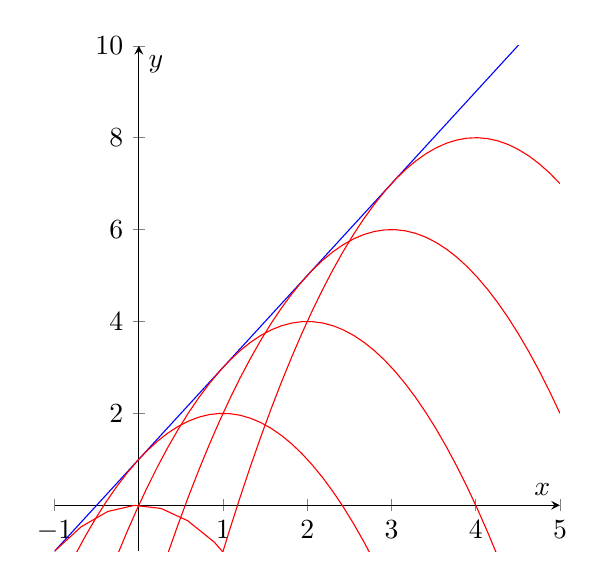
\begin{tikzpicture}
    \begin{axis}[
      width=8cm, height=8cm,
      axis lines=middle,
      xlabel={$x$}, ylabel={$y$},
      xmin=-1, xmax=5,
      ymin=-1, ymax=10
  	]
    	\addplot[domain=-1:5, samples=20, color=blue]{2*x+1}; % Enveloping function
			\addplot[domain=-1:5, samples=20, color=red]{-(x^2)}; % t=0
			\addplot[domain=-1:5, samples=50, color=red]{2-(x-1)^2}; % t=1
			\addplot[domain=-1:5, samples=50, color=red]{4-(x-2)^2}; % t=2
			\addplot[domain=-1:5, samples=50, color=red]{6-(x-3)^2}; % t=3
			\addplot[domain=-1:5, samples=50, color=red]{8-(x-4)^2}; % t=4
  	\end{axis}
	\end{tikzpicture}
\end{center}

We can see that the curve $y=2x+1$ is a tangent line to each of the cross=sections. In this case, $y=2x+1$ is an envelope for a family of one-variable functions. \\

The envelope, in general, is a curve which has the property that it is tangential to each cross-section at some point. The derivative of $y^{(t)}(x)$ is simply
$$
	\dyd[y^{(t)}]{x} = f_x(x,t).
$$
Let $t=g(x)$ be a solution (if it exists) of $f_t(x,g(x))=0$. Then define the evelope $E(x)$ to be
$$
	E(x) = f(x,g(x))
$$
The curve $E(x)$ intersects the cruve $y^{(t*)}(x)$ at the point $x_0$ whenever $t*=g(x_0)$. Moreover, these curves have the same derivative at $x_0$.

\ex{}{
	Show that the enveloping function of $f(x,t)=2t-(x-t)^2$ is $y=2x+1$.
	\begin{align*}
		y^{(t)}(x) &= f(x,t) \\
		\del{f}{t} &= 2 + 2(x-t) = 2 + 2x - 2t \\
		\Let f_t(x,t) &= 0 \\
		\Then 2 + 2x - 2t &= 0 \\
		1 + x - t &= 0 \\
		1 + x &= t \\
		\Substitute t = g(x) = x + 1 &\to f(x,t) \\
		f(x,g(x)) &= 2(x+1) - (x - x - 1)^2 \\
			&= 2x+2 - 1 \\
			&= 2x+1 \\
		\tf E(x) &= f(x,g(x)) = 2x+1
	\end{align*}
}

\section{Lecture 16}
\subsection*{Line Integrals}
Say we have a curve in $\bbr^3$ parametrised by
$$
	x=x(t),\qquad y=y(t),\qquad z=z(t),\qquad a\leq t\leq b.
$$
In other words, $\ut{r}(t) = (x(t), y(t), z(t)),\ t\in[a,b]$. We can work out the arc length of such a curve. Each individual segment of the arc length can be approximated,
$$
	\D s_i \approx \abs{\abs{\dyd[\ut{r}]{t}}}_{t=t_i}\D t_i
$$
The arc length, $S$ will be the sum of all these segments, namely,
$$
	S = \sum_{i=1}^{n}\D s_i \approx \sum_{i=1}^{n}\D t_i \abs{\abs{\dyd[\ut{t}]{t}}}_{t=t_i}
$$
If we take the limit, as $n\to\infty$ of the expression, $\D t\to0$ and $\D s\to0$, and we see
$$
	S = \int_a^b \abs{\abs{\dyd[\ut{r}]{t}}}\d t = \int_{a}^{b} \sqrt{\bracks{\dyd[x]{t}}^2 + \bracks{\dyd[y]{t}}^2 + \bracks{\dyd[z]{t}}^2}\d t
$$
We use new notation to describe this, 
$$
	S = \int_{C}\d s \implies \d s = \abs{\abs{\dyd[\ut{r}]{t}}}\d t
$$
The line integral over $C$. In general, if $f(x,y)$ is defined on a smooth curve $C\in\bbr^2$ then the line integral of $f$ over $C$ is 
$$
	\int_C f(x,y)\d s
$$
If $C$ is parametrised by $\ut{r}(t),\ t\in[a,b]$ and $f(x,y)>0$, then this line integral gives the ribbon area under $f$ along $C$. Line integrals are generaltisations of one-dimensional definite integrals.

\ex{}{
	Find the length of the helix described by 
	$$
		\left\lbrace\begin{array}{l} x = \cos 10t \\ y = \sin 10t \\ z = t \end{array}\right.,\qquad t\in[0,\pi]
	$$
	\begin{gather*}
		\ut{r}(t) = (\cos(10t), \sin(10t), t) \Rightarrow \dyd[\ut{r}]{t} = (-10\sin(10t), 10\cos(10t), 1) \\
		\dyd[s]{t} = \abs{\abs{\dyd[\ut{r}]{t}}} = \sqrt{100\sin^2(10t) + 100\cos^2(10t) + 1} = \sqrt{100(\sin^2(10t) + \cos^2(10t))+1} = \sqrt{101} \\
		\tf S = \int_C\d s = \int_{0}^{\pi} \sqrt{101}\d t = \left.\sqrt{101}t\right|_{0}^{\pi} = \pi\sqrt{101} - 0\sqrt{101} = \pi\sqrt{101}
	\end{gather*}
}

\ex{}{
	Find the arc length of a semicircle of radius 2.
	\begin{gather*}
		\ut{r} = (2\cos t, 2\sin t),\ t\in[0,\pi] \\
		\dyd[\ut{r}]{t} = (-2\sin t, 2\cos t) \\
		\abs{\abs{\dyd[\ut{r}]{t}}} = \sqrt{4\sin^2 t + 4\cos^2 t} = 2 \\
		\tf S = \int_C \d s - \int_{0}^{\pi} 2\d t = \left. 2t \right|_{0}^{\pi} = 2\pi
	\end{gather*}
}

\section{Lecture 17}
\subsection*{Polar Curves}
A polar curve is the set of points whose polar coordinates satisfy
$$
	r = f(\theta)
$$
Here, $r$ is the distance from the origin, and $\theta$ is the angular displacement from the positive $x$ axis. Any polar curve can be parametrised as
$$
	r = f(\theta) \implies \begin{array}{l} x(\theta) = f(\theta)\cos\theta \\ y(\theta) = f(\theta)\sin\theta \end{array}\qquad\text{or}\qquad \ut{r}(\theta) = f(\theta)\cos(\theta)\ihat + f(\theta)\sin(\theta)\jhat,\ \theta\in[\alpha,\beta]
$$
For a polar curve, the arc length is expressed
$$
	S = \int_\alpha^\beta \sqrt{f'(\theta)^2 + f(\theta)^2}\ \d\theta.
$$
We find this by differentiating $\ut{r}$ with respect to $\theta$ and finding the square of the magnitude. We end up canceling a bunch of the trigonometric functions, which square and sum to give 1. All thats left over is the root of the sum of the function squared and its derivative squared.

\subsection*{Word Done by a Constant Force}
In one dimension, the work done by a constant force, $F$, along a straight line of length $d$ is $W = Fd$. \\

In two dimensions, the work done by a constant force in moving a particle along a straight line from $P$ to $Q$ is $W = \ut{F}\cd\overrightarrow{PQ}$. This is because only the component of $F$ which is perpendicular to $\overrightarrow{PQ}$ is contributing to work done. This, in essence, transforms our 2 dimesnionsal problem, back into a one dimensional problem. Where $\theta$ is the angle from $\overrightarrow{PQ}$ to $\ut{F}$,
$$
	W = \Mag{\ut{F}}\cos\theta \cd \Mag{\overrightarrow{PQ}} = \ut{F}\cd\overrightarrow{PQ}
$$

\subsection*{Word Done Over a Curve}
Lets now consider a more general case of work done by an object, through a force field.
$$
	\ut{F}(x,y,z) = F_1(x,y,z)\ihat + F_2(x,y,z)\jhat + F_3(x,y,z)\khat
$$
where $F_1,F_2,F_3$ are continuous functions, and the object moves along a curve $C$. \\

Similarly to how we defined the line integral initally, we start by chopping up $C$ into $N$ finite pieces, and observing that the work done by the $i$th line segment is 
$$
	W_i \approx \ut{F}(P_i) \cd \ut{T}(P_i) \D s_i,
$$
where $P_i$ is the $i$th sample point, $\ut{T}$ is a vector functoin, which is the unit vector tangent to $C$, and $\ut{F}$ is a vector function which is the value of the vector field at the sample point. The dot product represents the $\ut{F}$ component tangent to $C$ at the sample point, and $\D s_i$ is a scale factor, the distance from the start to the end of the segment. The total work done, is the sum of all these segments,
$$
	W \approx \sum W_i = \sum_{\forall i} \ut{F}(P_i)\cd\ut{T}(P_i) \D s_i.
$$
Just as before, we take the limit as the number of segments goes to infinty, or as the segment distance goes to 0, and observe that
$$
	W = \int_C \ut{F}\cd\ut{T}\d s
$$
To evaluate the line integral, we use a parameterisation of the curve $C$. Let $C$ be parameterised by
$$
	\ut{r}(t) = (x(t), y(t), z(t)),\ t\in[a,b]
$$
We can write $\ut{T}$ in terms o this parameterisation, 
$$
	\ut{T}(P_i) = \frac{\ut{r}'(t_i)}{\Mag{\ut{r}'(t_i)}}.
$$
Hence the work done over the $i$th arc is approximately
$$
	W_i \approx \ut{F}(\ut{r}(t_i))\cd\ut{r}'(t_i)\D t
$$
Summing up all these arcs gives us
$$
	W \approx \sum_{\forall i} W_i = \sum_{\forall i} \ut{F}(\ut{r}'t_i))\cd\ut{r}'(t_i)\D t.
$$
Finally, we take the limit as $\D t\to 0$,
$$
	W = \int_a^b \ut{F}(\ut{r}(t))\cd\ut{r}'(t)\ \d t.
$$
This line integral is commonly expressed
$$
	\int_C \ut{F}\cd\d\ut{r}
$$
but this is merely a notational convenience, you could consider 
$$
	\d\ut{r} = \d x\ihat + \d y\jhat + \d z\khat
$$
but again, this is just a notational convenience, and only really serves to remind us where this formula came from.

\ex{}{
	Evaluate $\int_C \ut{F}\cd\d\ut{r}$ where $\ut{F}=(xy,yz,zx)$ and $C$ is parameterised $x=t$, $y=t^2$, and $z=t^3$, $t\in[0,1]$.
	\begin{gather*}
		\ut{r}(t) = (x(t), y(t), z(t)) = (t, t^2, t^3) \\
		\tf\ut{r}(t) = (1, 2t, 3t^2) \\
		\ut{F}(\ut{r}(t)) = (x(t)y(t), y(t)z(t), z(t)x(t)) = (t^3, t^5, t^4) \\
		\tf\ut{F}(\ut{r}(t)) \cd \ut{r}'(t) = (1\cd t^3) + (2t\cd t^5) + (3t^2\cd t^4) = t^3 + 2t^6 + 3t^6 = t^3 + 5t^6 \\
		\tf\int_C\ut{F}\cd\d\ut{r} = \int_0^1 t^3 + 5t^6\ \d t = \left. \frac{1}{4}t^4 + \frac{5}{7}t^7 \right|_0^1 = \frac{27}{28}
	\end{gather*}
}

\chapter{Week 7}
\section{Lecture 18}
\subsection*{Conservative Fields}
Gradient fields are a type of force field with a special property of being \textit{conservative}. There is a relatively easy way to determine if a field is conservative. \\

Let $A$ and $B$ be points, then if $\int_A^B \ut{F}\cd\d\ut{r}$ is independent of the path taken (that is, forall paths connected the points $A$ and $B$, the result is the same), then $\ut{F}$ is called a conservative field. \\

That is, if $\ut{F}$ is conservative, then all paths connecting $A$ and $B$ will give the same result. \\

If there exists a function $f(x,y)$ such that $\ut{F} = \grad f$, then $\ut{F}$ is a gradient field, with a potential function $f$. All gradient fields are conservative, and if you can find a potential function, then
$$
	\int_A^B \ut{F}\cd\d\ut{r} = f(B) - f(A)
$$
\nt{
	This equation is really important!!
}

\ex{}{
	Show that $\ut{F}(x,y) = (x+y, x+1)$ is a gradient field.
	\begin{align*}
		\grad f &= \bracks{\del{f}{x}, \del{f}{y}} \\
		\del{f}{x} &= x + y \\
		\Rightarrow f(x,y) &= \int\del{f}{x}\d x \\
			&= \frac{1}{2}x^2 + xy + g(y) \\
		\del{f}{y} &= x+1 \\
			&= \del{}{y}\bracks{\frac{1}{2}x^2 + xy + g(y)} \\
			&= x + g'(y) \\
		\Rightarrow g'(y) &= 1 \\
		\Rightarrow g(y) &= y \\
		\tf\bracks{f(x,y): \ut{F}=\grad f} &= \frac{1}{2}x^2 + xy + y
	\end{align*}
}

\ex{}{
	Show that $\ut{F} = \frac{x + y}{2}\ihat + \frac{1}{2}y\jhat$ is not a gradient field.
	\begin{align*}
		\Suppose \exists f(x,y) : \ut{F} = \grad f &\phantom{=} \\
		\Then \del{f}{x} &= \frac{1}{2}xy \\
		\Rightarrow f &= \int \del{f}{x}\d x \\
			&= \int \frac{1}{2}x + \frac{1}{2}y\ \d x \\
			&= \frac{1}{4}x^2 + \frac{1}{2}xy + g(y) \\
		\del{f}{y} &= \del{}{y}\bracks{\frac{1}{4}x^2 + \frac{1}{2}xy + g(y)} \\
			&= \frac{1}{2}x + g'(y) \\
			&= \frac{1}{2}y	\tag*{\contra} \\
		\because g'(y) &= \frac{1}{2}y - \frac{1}{2}x \tag*{\contra} \\
		\tf\nexists f(x,y) : \ut{F} = \grad f &\phantom{=}
	\end{align*}
}

It turns out that you don't need to find a potential function to check if a force field $\ut{F}=(F_1,F_2)$ is a gradient field. If $\ut{F}$ is a gardient field,
$$
	\del{F_1}{y} = \del{F_2}{x}
$$

\section{Lecture 19}
\subsection*{Conservation of Energy in Three-Dimensional Space}
We've seen that if $\ut{F}$ is conservative, $\ut{F}=\grad f$. Take $V(\ut{r}) = -f(\ut{r})$. By Newton's Second Law,
$$
	\ut{F} = -\grad V = m\ut{\ddot{r}}
$$
where $\ut{\ddot{r}}$ is the second derivative of position with respect to time, ie, acceleration. We can then apply the dot product of $\ut{\dot{r}}$ to both sides:
$$
	-\grad V\cd\ut{\dot{r}} = m\ut{\ddot{r}}\cd\ut{\dot{r}}
$$
Let's now analyse the LHS
\begin{align*}
	LHS &= -\bracks{\del{V}{x}, \del{V}{y}, \del{V}{z}}\cd\bracks{\dyd[x]{t}, \dyd{t}, \dyd[z]{t}} \\
		&= -\bracks{\del{V}{x}\dyd[x]{t} + \del{V}{y}\dyd{t} + \del{V}{z}\dyd[z]{t}} \\
		&= -\dyd[V]{t}
	\intertext{Now the RHS}
	RHS &= m\ut{\ddot{r}}\cd\ut{r} \\
		&= m\bracks{\dyd[^2x]{t^2}, \dyd[^y]{t^2}, \dyd[^z]{t^2}}\cd\bracks{\dyd[x]{t}, \dyd{t}, \dyd[z]{t}} \\
		&= m\bracks{\dyd[^2x]{t^2}\dyd[x]{t} + \dyd[^y]{t^2}\dyd{t} + \dyd[^z]{t^2}\dyd[z]{t}} \\
		&= \frac{m}{2}\dd{t}\bracks{\bracks{\dyd[x]{t}}^2 + \bracks{\dyd[y]{t}}^2 + \bracks{\dyd[z]{t}}^2} \\
		&= \frac{m}{2}\dd{t}\Mag{\ut{\dot{r}}(t)}^2
	\intertext{Hence the second law of motion becomes}
	-\dyd[V]{t} &= \frac{m}{2}\dd{t}\Mag{\ut{\dot{r}}(t)}^2 \\
	0 &= \dd{t}\bracks{\frac{m}{2}\Mag{\ut{\dot{r}}(t)}^2 + V(\ut{r}(t))} \\
	E &= \frac{m}{2}\Mag{\ut{\dot{r}}(t)}^2 + V(\ut{r}(t))
	\intertext{where $E$ is constant, introduced in the integration in the final step.}
\end{align*}
This is the energy equation. The first term is a function of velocity. It is the contribution to the total energy due to the object's motion, and is called kinetic energy (K.E.). Note that $\Mag{\dyd[\ut{r}]{t}}^2\geq0$, so kinetic energy is non-negative. \\

The second term is a function of poistion, called potential energy (P.E.), because it has the potential to be converted to kinetic energy.

\subsection*{Central Forces}
A force is called central if it has the form:
$$
	\ut{F} = F(r)\unit{r} = \frac{F(r)}{r}\ut{r}
$$
where $\ut{r}(t) = x\ihat + y\jhat + z\khat$ and $r = \Mag{\ut{r}}$. \\

The magnitude of a central force is dependent only on the distance of the object from the origin. Such a force is called attractive if it acts towards the origin ($F(r) < 0$), and repulsive if it acts away from the origin ($F(r) > 0$).

\thm{}{
	If $F(r)$ is continuous over some domain $D$, then the central field $\ut{F}=F(r)\unit{r}$ is conservative throughout $D$.
}
\proof
\begin{gather*}
	\intertext{Consider the gradient of the radial distance}
	\grad\ut{r} = \dyd[r]{x}\ihat + \dyd[r]{y}\jhat + \dyd[r]{z}\khat
		= \frac{x}{r}\ihat + \frac{y}{r}\jhat + \frac{z}{r}\khat = \frac{1}{r}\bracks{x\ihat + y\jhat + z\khat} 
		= \frac{\ut{r}}{r}
		= \unit{r}
	\intertext{Let $f(r)$ be the anti derivative of $F(r)$. ie, $F(r)=f'(r)$. Since $F$ is continuous, $f$ must exist.}
	\grad f(r) = \del{f}{x}\ihat + \del{f}{y}\jhat + \del{f}{z}\khat
		= \dyd[f]{r}\del{r}{x}\ihat + \dyd[f]{r}\del{r}{y}\jhat + \dyd[f]{r}\del{r}{h}\khat = \dyd[f]{r}\bracks{\del{r}{x}\ihat + \del{r}{y}\jhat + \del{r}{z}\khat} = f'(r)\grad\ut{r} = F(r)\unit{r}
	\longintertext{Therefore, the central force $\ut{F}$ is a gradient field (hence conservative) with potential function $f(r)$. \\ Now, we set}
	V(r) = -f(r),\qquad \implies \ut{F}(\ut{r}) = -\grad V(r)
\end{gather*}

\subsection*{Angular Momentum}
Consider a particle with mass $m$, velocity $\ut{v}$ and position $\ut{r}$, we say its angular momentum is
$$
	\ut{L} = m(\ut{r}\times\ut{v})
$$
If force is exerted on a particle and we consider Newton's Second Law, $\ut{F} = m\ut{a}$,
$$
	\ut{\dot{L}} = \dd{t}\bracks{m(\ut{r}\times\ut{v})} = m\bracks{\ut{\dot{r}}\times\ut{v} + \ut{r}\times\ut{\dot{v}}} = m\bracks{\ut{v}\times\ut{v} + \ut{r}\times\ut{a}} = \ut{r}\times m\ut{a} = \ut{r}\times\ut{F}
$$
We call $\ut{r}\times\ut{F}$ torque.

\thm{}{
	Under all central forces, the angular momentum $\ut{L}$ is conserved.
}
\proof
\begin{gather*}
	\intertext{Recall that for a central force}
	\ut{F} = \frac{F(r)}{r}\ut{r} \\
	\ut{\dot{L}} = \ut{r}\times\ut{F} = \ut{r}\times\bracks{\frac{F(r)}{r}\ut{r}} = \frac{F(r)}{r}\bracks{\ut{r}\times\ut{r}} = \ut{0}
\end{gather*}
This is to say, that at all times, angular momentum, $\ut{L}$ does not change, it is conserved. Thus, central forces conserve both energy, and anuglar momentum.

\section{Lecture 20}
\thm{}{
	If a central force acts on an object in three dimensions, its motion is restricted to a plane.
}
Consider the plan $P$ upon which the inital position vector, $\ut{r}_0=\ut{r}(t_0)$, and inital velocity vector, $\ut{v}_0=\ut{v}(t_0)$, lie. Since $\ut{L} = m(\ut{r_0}\times\ut{v_0})$, $\ut{L}$ is perpendicular to $P$. \\

Since $\ut{L}$ is conserved, consider the vectors $\ut{r}_1=\ut{r}(t_1)$ and $\ut{v}_1=\ut{v}(t_1)$,
$$
	\ut{L} = m(\ut{r}_0\times\ut{v}_0) = m(\ut{r}_1\times\ut{v}_1)
$$
Since $\ut{r}_1$ and $\ut{v}_1$ are orthognal to $\ut{L}$ they must therefore also lie in $P$.

\subsection*{Position-Dependent Unit Vectors for Central Force Fields}
The acceleration of an object in a central force field depends only on the radial distance $r$. For central orce problems, we use polarcoordinates in $\bbr^2$
$$
	\begin{array}{c}
		x = r\cos\theta \\ y = r\sin\theta
	\end{array}
$$
We can express the position vector in a different way. $\theta$ is the angle between $\ut{r}$ and the $x$-axis.
$$
	\begin{array}{rll}
		\ut{r} & = & x\ihat + y\jhat \\
			& = & r\cos\theta\jhat + r\sin\theta\jhat \\
			& = & r(\cos\theta\jhat + \sin\theta\ihat) \\
			& = & r\unit{r}
	\end{array}
$$
Another unit vector is given by
$$
	\unit{\theta} = -\sin\theta\ihat + \cos\theta\jhat
$$
This $\unit{\theta}$ is perpendicular to $\unit{r}$
$$
	\unit{r}\cd\unit{\theta} = (\cos\theta\cd-\sin\theta + \sin\theta\cd\cos\theta) = 0
$$
and
$$
	\unit{r}\times\unit{\theta} = \begin{vmatrix} \ihat & -\jhat & \khat \\ \cos\theta & \sin\theta & 0 \\ -\sin\theta & \cos\theta & 0 \end{vmatrix} = \khat
$$
So, the vectors $\unit{r}$ and $\unit{\theta}$ form a basis for $\bbr^2$. Because these vectors are both orthognal and normal, we call them ``orthonormal,'' which is kinda cute. Unlike the $x$-$y$ Cartesian system we're used to, this co-ordinate system varies with the angle the particle makes with the $x$-axis. We can also expand these coordinates into concepts of position, velocity and anular momentum.
\begin{align*}
	\ut{r} &= r\unit{r} \\
		&= r(t)\unit{r}(\theta(t)) \\
	\ut{v} = \ut{\dot{r}} &= \dot{r}\unit{r} + r\dd{t}\unit{r}\dot{\theta} \\
		&= \dot{r}\unit{r} + r\dot{\theta}\unit{\theta} \\
	\ut{L} &= m(\ut{r}\times\ut{v}) \\
		&= m(r\unit{r})\times(\dot{r}\unit{r}+r\dot{\theta}\unit{\theta}) \\
		&= mr^2\dot{\theta}\unit{\theta}
\end{align*}

\subsection*{Motion in a Gravitational Field}
It can be shown that the trajectory of an object of mass $m$ in the gravitational system is given by the polar curve
$$
	r = \frac{l}{1 + e\cos\theta}
$$
This is an equation for a conic section, symmetric about the $x$-axis. Thus we conclude 
\begin{quote}\begin{center}
	The orbits of all objects acting under such a gravitational field must be conic sections, either circle, ellipse, parabola, or branch-hyperbola, with a focus at the origin.
\end{center}\end{quote}
This is called Kepler's First Law of Planetary Motion.
\nt{This won't be on the final exam, so we'll leave it at that. We could show that all gravitational orbits are conic sections, Stewart, ed.8 p916-917 for additional reading. For now, though, we'll just move on to ODEs ;)}

\chapter{Week 8}
\section{Lecture 21}
\subsection*{Ordinary Differential Equations}
Differential equations (DEs) is an equation which consists one or more derivatives of an unknown function. There are two types of DEs:
\begin{itemize}
	\item (ODEs) Ordinary DEs, where the unknown function is a function of only one variable.
	\item (PDEs) Partial DEs, where the unknown function is a function of more than one variable. We will not consider PDEs at all in this class.
\end{itemize}
In ODEs, one often takes time, $t$, as the independent variable, instead of $x$. Also derivatives such as $x'(t)$ and $x''(t)$ with respect to time, are often denoted $\dot{x}$ and $\ddot{x}$.\\

Some examples of ODEs:
\begin{itemize}
	\item Unbounded population growth: $P'(t) = kP$
	\item Motion due to gravity: $mx''(t) = -kx$
	\item Spring system: $mx''(t) = -kx$
	\item Interaction between electric charges: $r'' = Kr^{-2}$
	\item General form of linear ODEs: $y^{(n)} = f(x, y', y'', \dots y^{(n-1)})$
\end{itemize}
We will only study linear ODEs in this course.

\subsection*{Solution to an ODE}
Suppose we are given an ODE for $y$ which is an unknown function of $x$. Then $y=f(x)$ is said to be a solution to the ODE if the ODE is satisfied when $y=f(x)$ and its derivatives are substituted into the equation. \\

When asked to \textit{solve} an ODE, you are expected to find all possible solutions. This means that you need to find the general solution to the ODE. For an ODE that involves only the unknown function of $y$ and its first derivative, the general solution will involve one arbitrary constant.

\ex{}{
	Show that $y=A\exp(x^2/2)$ is a general solution to $y' = xy$.
	\begin{align*}
		y' &= xy \\
			&= x A\exp(x^2/2) \\
		xy &= x A\exp(x^2/2) \\
	\end{align*}
	Since LHS = RHS, $y=A\exp(x^2/2)$ is a general solution to $y'=xy$.
}

\ex{}{
	Find the general solutionn to the DE $y'=x^2$
	\begin{align*}
		y' &= x^2 \\
		\Rightarrow y &= \int y' \d x \\
			&= \int x^2 dx \\
			&= \frac{1}{3}x^3 + C,\ C\in\bbr
	\end{align*}
}

\subsection*{Order of an ODE}
The order of an ODE is defined by the highest order derivative present in the ODE
\begin{itemize}
	\item $\dyd[P]{t} = kP$: First Order
	\item $m\ddot{x} = -kx$: Second Order
	\item $x(y'')^2 + y'y''' + 4y^5 = yy'$: Third Order
	\item $y'=xy$: First Order
\end{itemize}

\subsection*{Inital Value Problem}
An IVP is the problem of solving and ODE subject to some inital conditions of the form $y(t_0) = a,\ y'(t_0) = b,$ etc. The solution to an IVP no longer contains any arbitrary constants, because they've been determined by the inital conditions. 

\ex{}{
	A flow-meter in a pipline measures flow-through as $2+\sin t$L/sec. How much fluid passes through the pipline from time 0 to time $t$.
	\begin{gather*}
		\dyd[V]{t} = 2 + \sin t,\quad \sqbracks{\dyd[V]{t}} = L^3T\inv,\quad \sqbracks{t} = T^1 \\
		\text{Let's introduce 2 varaibles:}\ \sqbracks{\omega} = T\inv,\quad \sqbracks{\alpha} = L^3T\inv
		\intertext{These varaibles enable the $\sin$ to be dimensionless, and for the RHS to match the dimensions of the LHS. With these variables, let us suggest a new model:}
		\dyd[V]{t} = \alpha\bracks{2 + \sin(\omega t)}
		\Rightarrow V = \int\dyd[V]{t}\d t = 2\alpha t - \frac{\alpha}{\omega}\cos(\omega t) + C,\ C\in\bbr \\
		V(0) = 0 = 0 - \frac{\alpha}{\omega}\cos0 + C \iff 0 = C - \frac{\alpha}{\omega} \iff C = \frac{\alpha}{\omega}
		\intertext{Therefore, the final solution is}
		V(t) = 2\alpha t - \frac{\alpha}{\omega}\cos(\omega t) + \frac{\alpha}{\omega}
	\end{gather*} 
}

\subsection*{Solution Curves}
We'll intoduce this with an example. Suppose we want to find the position of a bike, traveling at a constant 60km/hr, along a perfectly straight road, at time $t$. If $x=x(t)$ is the distance travelled at time $t$, the ODE is
$$
	\dyd[x]{t} = 60
$$
and we can find the solution by directly integrating,
$$
	x = \int \dyd[x]{t}\d t = \int 60\d t = 60t + C,\ C\in\bbr
$$
To determine that constant $C$, we need more information, like the inital position at time $0$. In such a case, we'd be solving the IVP. For different values of $C$, we'd find different solutions, suppose we graphed some of these solutions
\begin{center}
	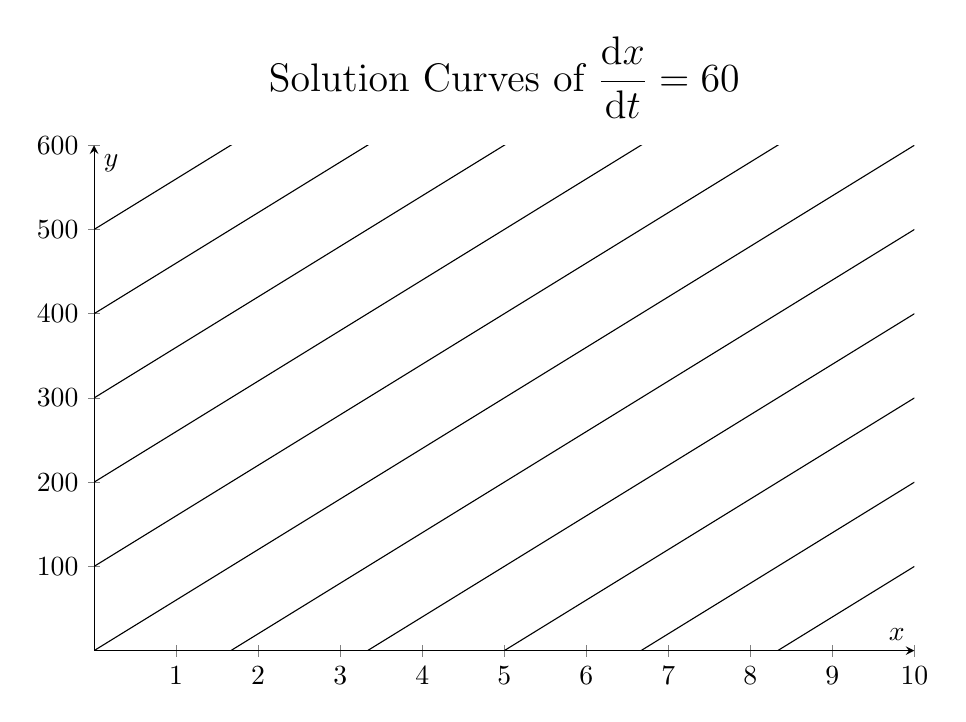
\begin{tikzpicture}
    \begin{axis}[
			title={\Large Solution Curves of $\dps{\dyd[x]{t} = 60}$},
      width=12cm, height=8cm,
      axis lines=middle,
      xlabel={$x$}, ylabel={$y$},
      xmin=0, xmax=10,
      ymin=0, ymax=600
  	]
    	\addplot[domain=0:10, samples=5, color=black]{60*x+0};
    	\addplot[domain=0:10, samples=5, color=black]{60*x+100};
  		\addplot[domain=0:10, samples=5, color=black]{60*x+200};
  		\addplot[domain=0:10, samples=5, color=black]{60*x+300};
  		\addplot[domain=0:10, samples=5, color=black]{60*x+400};
  		\addplot[domain=0:10, samples=5, color=black]{60*x+500};
  		\addplot[domain=0:10, samples=5, color=black]{60*x-100};
  		\addplot[domain=0:10, samples=5, color=black]{60*x-200};
  		\addplot[domain=0:10, samples=5, color=black]{60*x-300};
  		\addplot[domain=0:10, samples=5, color=black]{60*x-400};
  		\addplot[domain=0:10, samples=5, color=black]{60*x-500};
  	\end{axis}
	\end{tikzpicture}
\end{center}

These curves, $y=60t + C$ are called the solution curves to the ODE. Note that in this particular case, the solutions curves are all straight lines of slope 60.

\subsection*{Analytical and Numerical Solutions}
To solve an ODE (or IVP) analytically means to give a solution curve in terms of continuous functions defined over a specified interval, where the solution is obtained exactly by analytic means, for example, integration. The solution satisfies the ODE and inital conditions on direct substitution. \\

To solve an ODE or IVP numerically means to use an algorithm to generate a sequence of points which approximate a solution curve.

\section{Lecture 22}
\subsection*{Slope Fields}
We have seen that in order to solve
$$
	\dyd{t} = f(t)
$$
we only need to integrate. However, for the more general first-order ODE,
$$
	\dyd{t} = f(t,y)
$$
this doesn't work anymore. Nonetheless, the ODE gives a qualitative picture of the solution by noting at $(t,y)=(a,b)$ the slope of $y(t)$ is $f(a,b)$. So, as follows, we can
\begin{itemize}
	\item In the $ty$-plane at $(t,y)=(a,b)$ draw a small straight line with slope $f(a,b)$.
	\item Repeat this process for many different values of $(a,b)$.
	\item The resulting diagram is called the slope field.
\end{itemize} 
Note that the slope field can be generated without having to solve the ODE.

% TODO: SLOPE FIELD HERE

\subsection*{Equilibrium Solutions}
An equilibrium solution is a constant solution $y(t)=c$ to the ODE
$$
	\dyd{t} = f(t,y)
$$
The graph of an equilibrium solution is a horizontal line. Such a line has a slope of 0, $y'=0$, and only happens if $f(t,y)=0$ has a solution $y=c$ for some $c\in\bbr$.

\ex{}{
	Find the equilibrium solutions of $y'(t)=-3(y-1)$
	\begin{gather*}
		y'(t) = 0,\ \forall t \implies y(t) = c,\ \forall t \\
		y(t) = 1 \implies y'(0),\ \forall t \\
		\intertext{Consider the long term behaviour}
		y > 1 \implies y'(t)<0 \implies \text{decreasing solution} \\
		y < 1 \implies y'(t)>0 \implies \text{increasing solution} \\
		\implies \lim_{t\to\infty} y(t) = 1
	\end{gather*}
	No matter what the initial conditions are, in the long term, the system will settle at the equilibrium $y(t)=1$. This can be obsrved nicely on the slope field
}

% TODO: SLOPE FIELD HERE

\ex{}{
	Find the equilibrium solutions of $y'(t) = 2t + 1$
	\begin{gather*}
		\nexists c\in\bbr: \forall t,\ y'(t)=0 \implies \text{no equilibrium} \\
		\int y'(t)\d t = \int 2t + 1\d t = t^2 + t + c \\
		\intertext{Consider the long term behaviour}
		\lim_{t\to\infty} y(t) = +\infty
	\end{gather*}
	No matter what the inital conditions are, in the long term, the system will diverge positively. No equilibrium point.
}

% TODO: SLOPE FIELD HERE

\ex{}{
	Find the equilibrium solutions of $y'(t) = y(1-y)$
	\begin{gather*}
		\forall y'(t) = 0 \implies \forall t, y(t) = c,\ c\in\bbr \\
		y = 1,\ y= 0,\ \text{make equilibrium solutions} \\
		y'(t) = 0(1-0) = 1(1-1) = 0 \\
		\intertext{Consider the long term behaviour}
		y > 1 \implies y'<0 \implies \text{decreasing solution}\\
		0<y<1 \implies y'>0 \implies \text{increasing solution}\\
		y < 0 \implies y'<0 \implies \text{decreasing solution}
	\end{gather*}
	Long term behaviour depends on the inital conditions. If, for example, $y(0)=2$, then the system will settle at the equilibrium 1. If $y(0)=-2$, in the long term, the system will diverge negatively. 
}

\subsection*{Stability of Equilibrium Solutions}
A pencil sitting balanced vertically is in an equilibrium state. But make one small pertubrbation and it will topple. This is an unstable equilibrium. On the other hand, a pendulum hanging vertically is also in an equilibrium state. But if you perturb it slightly, it will eventually settle back down at its equilibrium point; this is a stable equilibrium. \\

From a slope field you can identify stable and unstable equilibriums by looking at if curves tend towards the equilibrium or away from it as time increases. \\

Formally, an equilibrium solution $y(t)=y_0$ to the DE $y' = f(t,y)$ is stable if the inital value problem:
$$
	\dyd{t} = f(t,y),\qquad y(0) = y_0 \pm\veps
$$
has a solution which satisfies
$$
	\lim_{t\to\infty}y(t) = y_0.
$$
In other words, if you start from sufficently close to a stable equilibrium, the you will approach that equilibrium solution.
\begin{itemize}
	\item Stable: All slopes sufficently close to the equilibrium converge to the equilibrium.
	\item Unstable: All slopes sufficently close to the equilibrium diverge from the the equilibrium.
	\item Semistable: Some slopes sufficently close to the equilibrium converge to the equilibrium.
\end{itemize}

% TODO: SLOPE FIELD HERE

\subsection*{Existence and Uniqueness of Solutions}
Consider the IVP
$$
	\dyd{t} = f(t,y),\qquad f(t_0) = y_0
$$
There exists a theorem asserting that, if $f(t,y)$ is smooth (that is continuous and first deriviatve is continuous) in some rectangle about $(t_0, y_0)$ there exists a unique solution $y=y_1(t)$ in some small neighbourhood of $(t_0, y_0)$.

\thm{}{
	Let $f$ and $\dyd[f]{y}$ be continuous in some rectangle $\alpha\leq t_0\leq\beta$ and $a\leq y \leq b$, which contains $(t_0, y_0)$. Then, in some interval $t_0-h\leq t_0 \leq t_0+h\ \in[\alpha,\beta]$, there is a unique solution $y(t)$ to the inital value problem.
}

An important consequence of this is that equilibrium solutions cannot be crossed by other solution curves. In fact, no solutions curves can cross each other because this would mean that in some point(s), $y'(t)$ has more than one value. Equilibrium solutions therefore partition the solution space.

\section{Lecture 23}
\subsection*{Euler's Method for Numerical Solutions to ODEs}
The method gives a simple approximation solution to an ODE and is closely related to the notion of a slope field.

\subsubsection*{Euler's Method using Tangent Lines}
The equation of the straight line with slope $m$ passes through the point $(t,y)=(a,b)$ is
$$
	y = b + m(t-a)
$$
Euler's method uses tangent lines as an approximation to solution curves. The tangent line to a solution curve $y'=f(t,y)$ at $(t_0, y_0)$ is 
$$
	y = y_0 + f(t_0, y_0)(t-t_0)
$$
This approximates the cruve when $t$ is close to $t_0$. Imagine then, a family of solution curves to the differential equation. We can calculate an approximate value for $y$ at some later time by taking lots of small steps in time. At each step we will use the tangent line to the solution through our current point. This is Euler's Method. \\

Using $\D t$ as the step size for the algorithm,
$$
	t_1 = t_0 + \D t,\quad t_2 = t_1 + \D t,\quad \dots,\quad t_n = t_{n-1} + \D t
$$
To then approximate the $y$ values,
$$
	y_1 = y_0 + f(t_0, y_0)\D t,\quad y_2 = y_1 + f(t_1, y_1)\D t,\quad \dots,\quad y_n = y_{n-1} + f(t_{n-1}, y_{n-1})\D t,
$$

\ex{}{
	Use Euler's Method with $\D t=0.2$ to approximate a solution to $y(0.6)$ for the IVP
	$$
		\dyd{t}=2t,\qquad y(0) = 0.	
	$$
	Compare your approximation to the real value
	\begin{gather*}
		t_0 = 0,\quad t_1 = t_0 + \D t = 0 + 0.2 = 0.2,\quad t_2 = 0.4,\quad t_3 = 0.6
		\intertext{Use Euler's Method to find a numerical solution}
		y_0 = y(0) = 0,\\
		y_1 = y_0 + f(t_0)\D t = 0 + (0.0)0.2 = 0,\\
		y_2 = y_1 + f(t_1)\D t = 0 + (0.4)0.2 = 0.08,\\
		y_3 = y_2 + f(t_2)\D t = 0.08 + (0.8)0.2 = 0.24 \\
		\tf y(0.6) \approx 0.24
		\intertext{Now let's find the analytical solution}
		\dyd{t} = 2t \implies y = \int\dyd{t}\d t = \int 2t\d t = t^2 + c \\
		y(0) = 0 = (0)^2 + c \iff c = 0 \\
		\tf y(t) = t^2 \implies t(0.6) = 0.36 \\ 
		\implies \veps = \abs{y_3 - y(0.6)} = 0.12
	\end{gather*}
}

This method becomes more accurate as $\D t$ becomes smaller, but this means that a larger number of steps are required to find the numerical solution. We could use MATLAB, for instance, to solve the previous example, but with $\D = 0.05$,

\begin{lstlisting}{matlab}
	t = 0:0.05:0.6;
	y(1) = 0;
	for i = 1:12
		y(i+1) = y(i) + 2*t(i)*0.05;
	end
	disp(y(13));
	plot(t, y, '-');
\end{lstlisting}
\verb|Output: 0.3300| $\implies \veps = \abs{y_{13} - y(0.6)} = 0.03$ which is clearly a more accurate approximation!

\ex{}{
	Consider the IVP
	$$
		\dyd{t} = \sin(ty),\qquad y(0) = 1
	$$
	Write MATLAB code to esitmate $y(2)$, using Euler's Method with step size $\D t = 0.01$. \\
}

\begin{lstlisting}{MATLAB}
	Dt = 0.1
	t = 0:Dt:2;
	y(1) = 1;
	for i = 1:length(t)-1
		y(i+1) = y(i) + sin(t(i)*y(i))*Dt;
	end
	y(end)
\end{lstlisting}
\verb|Output: 1.8243| \\

A particular issue can occur if the $\D t$ is too large. For instance, after a step, the approximation might have jumped over the equilibrium solution, which is not analytically correct. The whole calculation would need to be thrown out or adjusted at that point.


\chapter{Week 9}
\section{Lecture 24}
\subsection*{Heun's Method - An Extension of Euler's Method}
We can think about Euler's method in a different way. Instead of approximating the derivative from first principles, let us integrate the ODE from $t_n$ to $t_{n+1}$
\begin{gather*}
	\Suppose y-\phi(t),\ \text{is a solution to the IVP} \left\lbrace\begin{array}{l} y' = f(t,y) \\ y(t_0) = y_0 \end{array} \right. \\
	\int_{t_n}^{t_{n+1}} \dyd[\phi]{t}\d t = \int_{t_n}^{t_{n+1}} f(t, \phi(t))\d t
\end{gather*}
Geometerically, this integral can be represented as the area under the curve $f(t,\phi(t)))$, and this area can be approximated with triangles of width $\D t = t_{n+1} - t_n$ and height $f(t_n, \phi(t_n))$,
$$
	\phi(t_{n+1}) = \phi(t_n) + f(t_n, \phi(t_n))\D t \qquad\text{or}\qquad y_{n+1} = y_n + f(t_n, y_n)\D t
$$
Fundamentally though, we're using a rectangular approximation of the area, and better area approximating shapes are availible, trapeziums, for example. In that case, we replace the intergral with the average of the two endpoints:
$$
	\phi(t_{n+1}) = \phi(t_n) + \frac{\D t}{2}\bracks{f(t_n, \phi(t_n)) + f(t_{n+1}, \phi(t_{n+1}))}
$$
As before, replacing $\phi$ with $y$ leads to
$$
	y_{n+1} = y_n + \frac{\D t}{2}\bracks{f(t_n, y_n) + f(t_{n+1}, y_{n+1})}
$$
But clearly, this is problematic, since our formula for $y_{n+1}$ is dependent on itself. To get around this, we can use Euler's method to approximate $y_{n+1}$.
$$
	y_{n+1} = y_{n} + \frac{\D t}{2}\bracks{f(t_n, y_n) + f(t_{n+1}, \hat{y}_{n+1})}
$$
where, $\hat{y}_{n+1} = y_n + f(t_n, y_n)\D t$. This is called Heun's method.

\subsection*{Seperable First-Order ODEs}
This is one of several classes of ODEs we will study. It is very important to be skilled at identifying and solving this type of ODE. A first order ODE is seperable, if it can be written
$$
	\dydx = f(x) g(y)
$$
\begin{itemize}
	\item $\dydx = y(1-y)$: \textbf{Seperable}. $f(x) = 1,\ g(y) = y(1-y)$.
	\item $\dydx = \exp(x+y)$: \textbf{Seperable}. $f(x)=\exp(x),\ g(y)=\exp(y)$.
	\item $y' = \exp(x+y)^2$: \textbf{Unseperable}. $y' = \exp(x^2 + 2xy + y^2)$.
	\item $\dot{y} = \frac{ty + y}{t^2}$. \textbf{Seperable}. $f(t) = \frac{t+1}{t},\ g(y) = y$
	\item $\dyd{t} = ty + y^2$: \textbf{Unseperable}. $\dot{y}=(t+y)y$
\end{itemize}
We can solve seperable ODEs following these steps:
\begin{enumerate}
	\setcounter{enumi}{-1}
	\item Determine that the ODE is seperable; can be written $\dps{\dydx = f(x)g(y)}$.
	\item Rewrite the expression as $\dps{\frac{1}{g(y)}\dydx = f(x)}$
	\item Integrate both sides with respect to $x$: $\dps{\int\frac{1}{g(y)}\dydx \d x = \int f(x)\d x}$
	\item Note that the integral on the LHS is a substitution and hence replace it with $\dps{\int\frac{\d y}{g(y)} = \int f(x)\d x}$
	\item If we're lucky, one or both sides can actually be evaluated.
	\item If we're very lucky, we can explicitly express $y$ as a function of $x$. 
\end{enumerate}

\subsection*{Singular Solutions}
In step 1, we rewrite $y' = f(x)g(y)$ as 
$$
	\frac{1}{g(y)}\dydx = f(x)
$$
We can't divide by 0, so if $g(y)=0$ we have a problem. \\

If there is such an $a$ such that $g(a)=0$, then the ODE will have an equilibrium solution at $y(x)=a$. This is easy to check:
$$
	\dydx = f(x)g(y),\qquad \text{at a}\ \dydx = g(0)f(x) = 0\cd f(x) = 0
$$
Such a solution is called a singular solution, because it won't generally arise from an earlier step. We need to always check for singular/equilibrium solutions.

\section{Lecture 25}
\subsection*{Linear First-Order ODEs}
If you cannot solve a differential equation by seperation, the next plan of attack should be to test if it is linear and use integration factor method. \\

If a first order DE can be written in form
$$
	\dyd{t} + p(t)y = q(t)
$$
it is linear.
\begin{itemize}
	\item $y'=x$: \textbf{Linear}. $p(x)=0,\ q(x)=x$
	\item $y'=\log x$: \textbf{Linear}. $p(x)=0,\ q(x)=\log x$
	\item $y'=y^2$: \textbf{Non-linear}.
	\item $y'=y$: \textbf{Linear}. $p(x)=1,\ q(x)=0$
	\item $y'y=1$: \textbf{Non-linear}.
	\item $y'=y+3\sin x$: \textbf{Linear}. $p(x)=-1,\ q(x)=3\sin x$
	\item $y'=t^5-t^2y$: \textbf{Linear}. $p(x)=t^2,\ q(x)=t^5$
	\item $y'=\sin y+e^x$ \textbf{Non-linear}.
	\item $\bracks{y'}^2=y$: \textbf{Non-linear}.
\end{itemize}
In general, let $\fkl=\dps{\dd{t} + p(t)}$ be a differential operator so that applying $\fkl[y],\ y\in C^1(\bbr)$
$$
	\fkl[y] = \dd{t}y + p(t)y
$$
\Defin{Linear} $\forall \alpha,\beta\in\bbr,\ y_1,y_2\in C^1(\bbr),\ \fkl[\alpha y_1 + \beta y_2] = \alpha\fkl[y_1] + \beta\fkl[y_2]$. \\
\Claim $\fkl$ is linear. 
\proof 
\begin{align*}
	\fkl[\alpha y_1 + \beta y_2] &= \dd{t}(\alpha y_1 + \beta y_2) + p(t)(\alpha y_1 + \beta y_2) \\
		&= \alpha\dd{t}y_1 + \beta\dd{t}y_2 + \alpha p(t)y_1 + \beta p(t)y_2 \\
		&= \alpha\dd{t}y_1 + \alpha p(t)y_1 + \beta\dd{t}y_2 + \beta p(t)y_2 \\
		&= \alpha\bracks{\dd{t}y_1 + p(t)y_1} + \beta\bracks{\dd{t}y_2 + p(t)y_2} \\
		&= \alpha\fkl[y_1] + \beta\fkl[y_2] \tag*{\qed}
\end{align*}

Now, recall the product rule for differentiation, written here in reverse
$$
	f\dyd[g]{t} + \dyd[f]{t}g = \dd{t}(fg)
$$
This formula is the key to solving first order linear ODEs

\ex{}{
	Solve $\dps{\dyd{t}+\bracks{\frac{2t}{t^2+1}}y = t^2 + 1}$
	\begin{gather*}
		\text{This ODE is linear,}\ p(t)=\frac{2t}{t^2+1},\ q(t)=t^2+1 \\
		\intertext{Multiply through by $\dps{(t^2+1)}$. This is called the intergrating factor, for future discussion.}
		(t^2+1)\dyd{t} + 2ty = (t^2+1)^2
		\intertext{This is just like the product rule! $\dps{f = t^2+1,\ \dyd[f]{t} = 2t,\ g=y,\ \dyd[g]{t} = \dyd{t}}$. So we can replace the entire LHS with the RHS of the product rule, as we've written it above.}
		\dd{t}\bracks{(t^2+1)y} = (t^2+1)^2
		\intertext{And now we can integrate both sides with respect to $t$ and cancel it on the LHS}
		\begin{aligned}
			\int\dd{t}\bracks{(t^2+1)y}\d t &= \int t^4 + 2t^2 + 1\ \d t \\
			\iff (t^2+1)y + c_2 &= \frac{t^5}{5} + \frac{2t^3}{3} + t + c_1 
		\end{aligned} \\
		\tf y = \frac{\frac{t^5}{5} + \frac{2t^3}{3} + t + c}{t^2+1},\quad c = c_1 - c_2 \in\bbr
	\end{gather*}
}

\subsection*{The Intergrating Factor}
Can we always multiply a first-order linear ODE by some function, such that the LHS matches the product rule? \\

Yes. \\

Given the ODE
$$
	\dyd{t} + p(t)y = q(t)
$$
we can multiply through by the yet-to-be-found intergrating factor $I(t)$:
$$
	I(t)\dyd{t} + I(t)p(t)y = I(t)q(t)
$$
We can think of $I$ as $g$, and $y$ as $f$, in the product rule above. Then the first term is $gf'$ and consequently we want the second term to be $fg' = yI'$. Since this term equals $Ipy$, we can infer that $I$ must satisfy the ODE
$$
	I'(t) = I(t)p(t)
$$
But this is a seperable ODE, which we already know how to solve!
$$
	I(t) = \exp\bracks{\int p(t)\d t}
$$

\section{Lecture 26}
\subsection*{Applications of First-Order ODEs}
\subsubsection*{Newton's Law of Cooling}
Newton's law of cooling states that the rate at which a body cools is proportional to the temperature difference between the body and its surrounding medium. \\

If $T$ is the temperature of the body and $T_m$ is the temperature of the surrounding medium, then, according to Newton's law
$$
	\dyd[T]{t} = -k(T-T_m),\qquad k > 0
$$
Here, the constant $k$ is chosen such that if $T > T_m,\ T'(t)$ is negative, describing cooling.

\subsubsection*{Electrical Engineering}
% TODO: ADD NOTES

\subsubsection*{Single-Species Population Models}
% TODO: ADD NOTES

\end{document}